\documentclass{source/Paper}

\begin{document}
    \tableofcontents
    %TODO 配合 ppt 看教材
    % https://www.yuque.com/xianyuxuan/coding/gez9yl#jRAxS
    \newpage
\section{Introduction}
    \newpage
\section{The Physical Layer}
最底层, network基础. 最小单位: bit. 不同 physical channels 决定 throughput, latency (delay) and error rate. 

\subsection{The theoretical basis for data communication}
\subsubsection{Fourier Series}
信息通过改变物理量来传输. 

Any reasonably behaved \textbf{periodic} function $g(t)=g(t+nT_0)$ with period $T$ can be represented as
\begin{align*}
    g(t)&=\sum_{n=-\infty}^{+\infty}a_n e^{j\textcolor{light_red}{2\pi fn}t}\\
    &=\sum_{n=-\infty}^{+\infty} a_n (\cos(\textcolor{light_red}{2\pi fn}t)+j\sin(\textcolor{light_red}{2\pi fn}t))
\end{align*}
where $f_0=\frac{1}{T_0}$ is \textbf{the fundamental frequency} of the periodic signal $g(t)$. 

If the period $T_0$ is known and the amplitudes an are given, the original periodic signal $g(t)$ can be reconstructed. 也可反求 $a_n$. 
\begin{align*}
    a_n=\frac{1}{T}\int_T g(t)e^{-j\textcolor{light_red}{2\pi fn}t}dt
\end{align*}


If $g(t)$ is a \textbf{real} signal, then the coefficient $a_{-n}$ is \textbf{the conjugate} of $a_n$.
\begin{align}
    g(t)&=C+\sum_{n=1}^{\infty}2A_n\cos (2\pi nft)+\sum_{n=1}^\infty 2B_n\sin (2\pi n ft)\\
    \notag A_n&=\frac{1}{T}\int_0^T g(t)\cos(2\pi nft)dt\\
    \notag B_n&=\frac{1}{T}\int_0^T g(t)\sin(2\pi nft)dt\\
    \notag C  &=\frac{1}{T}\int_0^T g(t)dt
\end{align}

但现实世界信号有限, 但可以假想为重复的无限信号, 如此可用 Fourier. 
%TODO P8 算一算

\subsubsection{Bandwidth-limited Signals}
信号在信道传输会衰减. 且信道对不同频率的影响不同. 但对某一根线, 振幅从0到$f_c$(the cutoff frequency, 截止频率)之前信号衰减很小. 

The width of the frequency range transmitted without being strongly attenuated is called the \textbf{bandwidth}(带宽). (带宽是没有大量衰减的范围) 带宽是物理属性, 不依赖于环境. 

\paragraph{Baseband Signals vs. Passband Signals}\quad
\begin{itemize}
    \item Signals that run from 0 up to a maximum frequency are called basedband signals.
    \item Signals are shifted to occupy a higher range of frequencies, such as in the case of all wireless transmission, are called passband signals.
\end{itemize}

$f_c$ carrier frequency

\paragraph{Bandwidth vs. Maximum Data Rate}
\begin{itemize}
    \item analogue bandwidth is a quantity measured in Hz.
    \item digital bandwidth is the maximum data rate of a channel, a quantity measured in bits/sec.
\end{itemize}
data rate 是使用 analogue bandwidth 最终传输结果. 


\subsubsection{The Maximum Data Rate of a Channel}
Channel Capacity --- the maximum rate at which data can be transmitted over a given communication path or channel under given conditions.

Four related concepts:
\begin{enumerate}
    \item Data rate (bps)
    \item Bandwidth (Hz)
    \item Noise
    \item Error rate
\end{enumerate}

\subsubsection{Nyquist Bandwidth}
在理想情况下的 the maximum signaling rate
\begin{align*}
    s(t)=\sum_n a_n g(t-nT)
\end{align*}
where $g(t)$ represents a basic pulse shape and $\{a_n\}$ is the binary sequence of $\{\pm 1\}$ transmitted at a rate of $\frac{1}{T}$ bits/s.

The optimal pulse shape: %(C 是 capacity, B 是 bandwidth) 
\begin{align*}
    g(t)=\frac{\sin 2\pi Bt}{2\pi Bt}
\end{align*}
\begin{itemize}
    \item Binary: \textcolor{light_red}{$C = 2B$} (V=2)
    \item Multilevel Signaling: \textcolor{light_red}{$C = 2B \log_2 V$} ($V$ is the number of discrete signal or voltage levels)
\end{itemize}
提升信号种类的数量可以提升data rate. 但提升有限度, 且会被在传输中的 noise and other impairment 限制. 

\subsubsection{Shannon Capacity}
仅假设白噪声, 不考虑其他影响, 仅理论最大值. SNR (信噪比)
\begin{align*}
    C&=B\log_2 (1+SNR)\\
    SNR_{dB}&=10\lg\frac{\text{signal power}}{\text{noise power}}=10\lg(SNR)
\end{align*}

\subsection{Three kinds of transmission media}
\subsubsection{Guided Transmission Media}
\begin{itemize}
    \item Persistent storage (固态存储)
    \item Twisted pairs (双绞线)
    \item Coaxial cable (同轴线缆)
    \item Power lines (交流电的线)
    \item Fiber optics (光纤)
\end{itemize}

\paragraph{Persistent storage} 卡车运硬盘仍是最高的 bandwidth. 但 delay 很大. 

\paragraph{Twisted pairs} 最古老但仍最常用的传输介质. 为什么要绞: 因为两根平行线会形成一个小天线, 纠缠会抵消其干扰. 一个信号是这两根线的电压差, 提升鲁棒性. 

\begin{figure}[!htb]
    \centering
    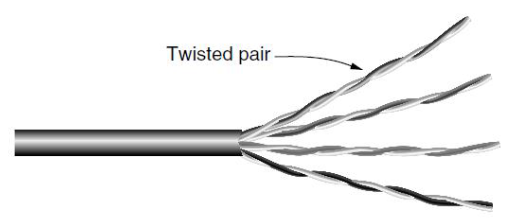
\includegraphics[width=0.309\textwidth]{pic/CN2/Twisted pairs.png}
    \caption{Twisted pairs}
\end{figure}

\paragraph{Coaxial Cable}黄铜轴x
\begin{figure}[!htb]
    \centering
    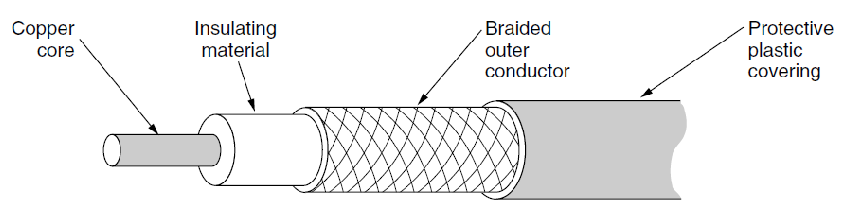
\includegraphics[width=0.42\textwidth]{pic/CN2/Coaxial Cable}
    \caption{Coaxial Cable}
\end{figure}

\paragraph{Power Lines}交流电的线. 中国民用交流电: 50Hz
\begin{figure}[!htb]
    \centering
    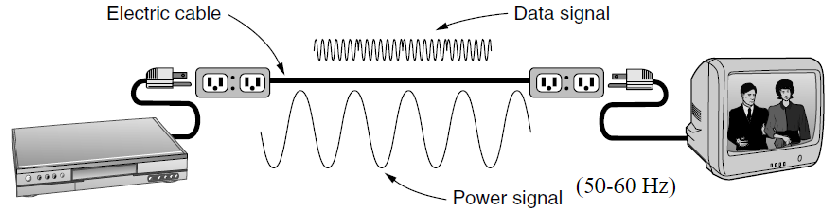
\includegraphics[width=0.42\textwidth]{pic/CN2/Power Lines}
    \caption{Power Lines}
\end{figure}

\paragraph{Fiber Optics}理论上 bandwidth可以无限大. 

重要组成部分: Light source, transmission medium, and detector. 

光源: LEDs, Semiconductor lasers.

\begin{figure}[!htb]
    \centering
    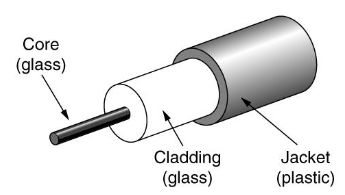
\includegraphics[width=0.309\textwidth]{pic/CN2/Fiber Optics}
    \caption{Fiber Optics}
\end{figure}

\subsubsection{Wireless}
three variations:
\begin{itemize}
    \item Frequency hopping spread spectrum
    \item Direct sequence spread spectrum e.g. CDMA
    \item UWB (Ultra WideBand)
\end{itemize}

\paragraph{Radio Transmission} Radio frequency (RF) waves 

\paragraph{Microwave Transmission} 传输是直线. 

\subsection{Digital modulation and multiplexing}
\subsection{Three examples of communication examples}
    \newpage
\section{Data Link Layer}
\subsection{Overview of Data link layer}
\subsubsection{The Design Principles of the Data Link Layer}

To achieve reliable and efficient communication between two adjacent machines

Three main functions of the data link layer:
\begin{itemize}
    \item Framing: Break stream of bits up into discrete frames
    \item Error control: Error Detection and Error Correction
    \item Flow control: to prevent a sender to overload the receiver with packets
\end{itemize}

\subsubsection{Position of the Data Link Layer}
\begin{figure}[!htb]
    \centering
    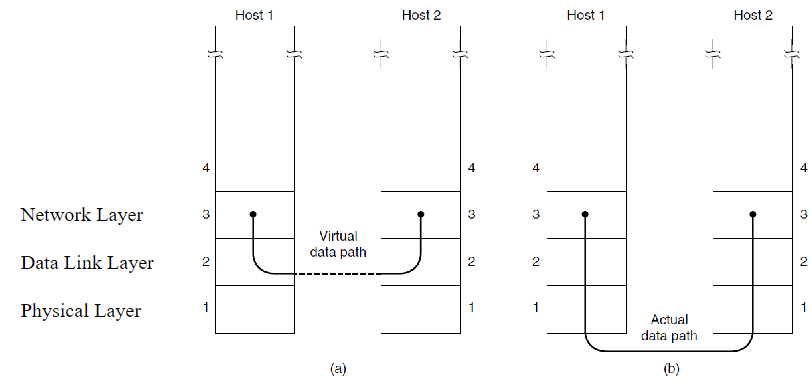
\includegraphics[width=0.42\textwidth]{pic/CN3/The function of the data link layer is to provide services to the network layer.}
    \caption{The function of the data link layer is to provide services to the network layer.}
\end{figure}

\subsubsection{The Services of Data Link Layer}
\begin{enumerate}
    \item Unacknowledged connectionless service
    \subitem for very low error-rate and real-time applications
    \subitem e.g. Ethernet
    \item Acknowledged connectionless service
    \subitem for unreliable channels
    \subitem e.g. 802.11 WiFi
    \item Acknowledged connection-oriented service
    \subitem for over long, unreliable links
    \subitem e.g. a satellite channel or a long-distance telephone circuit
\end{enumerate}

\subsection{Data link layer: Framing}
General Frame Format: a header, a payload field, and a trailer
\begin{figure}[!htb]
    \centering
    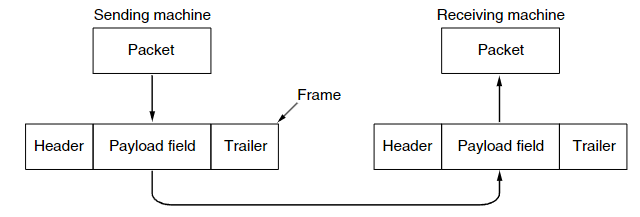
\includegraphics[width=0.42\textwidth]{pic/CN3/Relationship between packets and frames.}
    \caption{Relationship between packets and frames.}
\end{figure}

会加一些冗余的 bits 来降低 bit error rate. There are about four methods:
\begin{enumerate}
    \item Byte count: 若刚好 count 出错了就会很寄. 
    \item Flag bytes with byte stuffing: 因为 flag 可能会在传输数据中出现, 所以在其前加上 a special escape byte (ESC) 以区别, 若 ESC 也在数据中, 则同样其前加 ESC. 
    \begin{figure}[!htb]
        \centering
        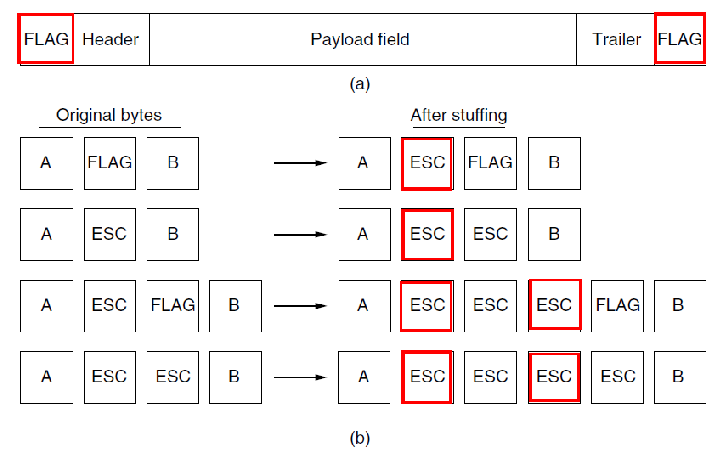
\includegraphics[width=0.42\textwidth]{pic/CN3/Flag Byte with Byte Stuffing.png}
        \caption{(a) A frame delimited by flag bytes. (b) Four examples of byte sequences before and after byte stuffing.}
    \end{figure}
    
    \item Flag bits with bit stuffing: Whenever the sender's data link layer encounters five consecutive 1s in the data, it automatically stuffs a 0 bit into the outgoing bit stream.
    \begin{figure}[!htb]
        \centering
        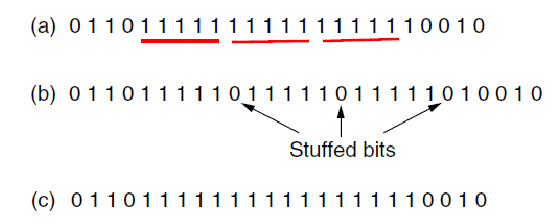
\includegraphics[width=0.309\textwidth]{pic/CN3/Flag Byte with Bit Stuffing.png}
        \caption{Bit stuffing. (a) The original data. (b) The data as they appear on the line. (c) The data as they are stored in the receiver's memory after destuffing.}
    \end{figure}
    
    \item Physical layer coding violations: We can use some reserved signals to indicate the start and the end frames.
\end{enumerate}

\subsection{Data link layer: Error Control}
\begin{itemize}
    \item Error-Correcting Codes: For unreliable channels
    \item Error-Detecting Codes: For highly reliable channels
\end{itemize}
the redundant bits that offer protection are as likely to be received in error as the data bits.

\subsubsection{Error Models of Communication Channels}

\subsubsection{Error Correction}
two different error-correcting codes:
\begin{itemize}
    \item Hamming codes
    \item Binary convolutional codes
\end{itemize}

对码本(一对码字), from this list to find the two codewords with the smallest Hamming distance. This distance is the Hamming distance of the complete code. (码本中码字间两两最小的 Hamming distance 是码本的 Hamming distance)

The code rate is $m/n$. (n=m+r, nis the total length of a block, r is redundance)

\begin{itemize}
    \item To reliably detect d errors, you need a distance d + 1 code
    \item To correct d errors, you need a distance 2d + 1 code.
\end{itemize}
we expect only single- or double-bit errors

For all single errors to be corrected, this requirement becomes
\begin{align*}
    (m+r+1)\le 2^r
\end{align*}
Given $m$, this puts a lower limit on the number of check bits needed to correct single errors. 

\paragraph{Hamming Code} $k$ data bits $+ (n - k)$ check bits. value 1 are XORed together to calculate the check bits.  %TODO 定义总结 P34-36

Convolutional Code: the original m bits do not appear % 不考, 摸了! P38-


\subsubsection{Error Detection}
three different error-detecting codes:
\begin{itemize}
    \item Parity: the number of 1 bits in the codeword is even or odd.
    \subitem Advantage: bit error rates 非常低时, 花费比 error correction 少
    \subitem Difficulty: for a long burst error (一大段错误), 仅能检测一般的错误. To against burst errors:
    \begin{itemize}
        \item Interleaving
        \begin{figure}[!htb]
            \centering
            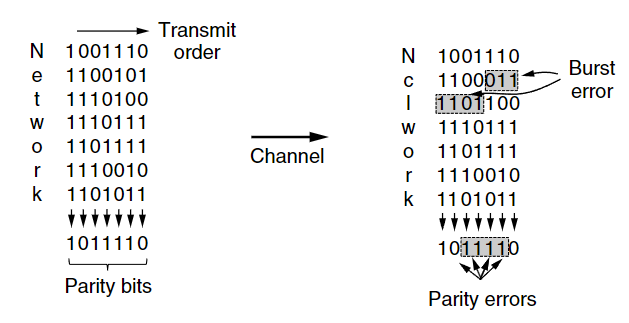
\includegraphics[width=0.309\textwidth]{pic/CN3/Interleaving}
            \caption{Interleaving of parity bits to detect a burst error}
        \end{figure}
        \item Two-dimensional parity
        \begin{figure}[!htb]
            \centering
            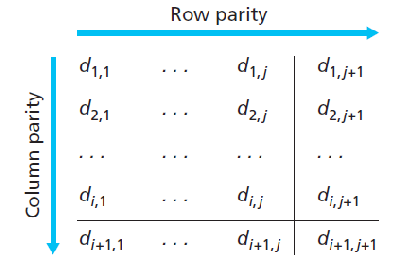
\includegraphics[width=0.309\textwidth]{pic/CN3/Two-dimensional parity}
            \caption{Two-dimensional parity}
        \end{figure}
        
    \end{itemize}
    \item Checksums: {\small
    \begin{itemize}
        \item One's complement has two representations of zero, all 0s and all 1s
        \item two's complement arithmetic
    \end{itemize}
    \subitem Sending:
    \begin{enumerate}
        \item Arrange data in 16-bit words
        \item Put zero in checksum position, add
        \item Add any carryover back to get 16 bits
        \item Negative (complement) to get sum
    \end{enumerate}
    \subitem Receiving
    \begin{enumerate}
        \item Arrange data in 16-bit words
        \item Checksum will be non-zero, add
        \item Add any carryover back to get 16 bits
        \item Negate the result and check it is 0.
    \end{enumerate} }
    \item Cyclic Redundancy Checks (CRCs): predetermined bit pattern - key (or the generator polynomial) (Both the high- and low-order bits of the generator must be 1)
    \begin{figure}[!htb]
        \centering
        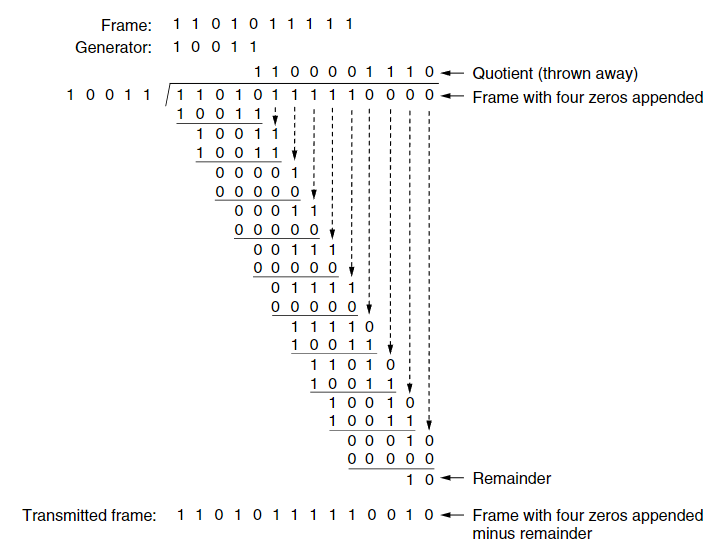
\includegraphics[width=0.309\textwidth]{pic/CN3/CRC.png}
        \caption{Example calculation of the CRC}
    \end{figure}
    
\end{itemize}


\subsection{Elementary data link protocols}
\subsubsection{A Utopian Simplex Protocol}
Unrealistic assumptions:
\begin{enumerate}
    \item Data are transmitted in one direction only.
    \item Both the transmitting and receiving network layers are always ready.
    \item Processing time can be ignored.
    \item Infinite buffer space is available.
    \item The communication channel between the data link layer never damages or loses frames.
\end{enumerate}

\subsubsection{A Simplex Stop-and-Wait Protocol for an Error-Free Channel}
This protocol is to tackle the problem of preventing the sender from flooding the receiver with frames faster than the latter is able to process them.

receiver provide a little dummy frame (an acknowledge frame) as feedback to sender (目的是告诉 sender, receiver 已完成接受).

\subsubsection{A Simplex Stop-and-Wait Protocol for a Noisy Channel}
To add a timer, the receiver would only send an acknowledgement frame if the data were correctly received. timer 触发但没收到 ack, sender 会重传. 

A fatal flaw: duplicate. 若 ack 完全丢失, 会接受一个 frame 两次, 不可接受. 

put a sequence number to avoid duplicate. the only ambiguity is between a frame and its immediate predecessor or successor

\begin{itemize}
    \item After transmitting a frame and starting the timer, the sender waits for something exciting to happen.
    \item Only three possibilities exist: an acknowledgement frame arrives undamaged, a damaged acknowledgement frame staggers in, or the timer expires.
\end{itemize}

\subsection{Sliding window protocols}
\subsubsection{Piggybacking(驮运)}
ack 可以搭顺风车, 与下一个数据包一起发送. The technique of temporarily delaying outgoing acknowledgements so that they can be hooked onto the next outgoing data frame. In effect, the acknowledgement gets a free ride on the next outgoing data frame.

使用一个计时器决定 ack 是否搭顺风车, 在时间内有其他包就顺风车, 没有就单独发. 

Sliding window bidirectional protocol(注意其不同点): 
\begin{itemize}
    \item A One-Bit Sliding Window Protocol (stop-and-wait)
    \item A Protocol Using Go Back N
    \item A Protocol Using Selective Repeat
\end{itemize}

\subsubsection{The Essence of All Sliding Window Protocols}
\paragraph{the sender}: maintains \textbf{a set of sequence numbers} corresponding to frames it is permitted to send. These frames are said to fall within the \textbf{sending window}.

The sequence numbers within the sender's window represents frames that 
\begin{enumerate}
    \item have been sent but are yet not acknowledged 
    \item can be sent
\end{enumerate}
(If some frames are lost or damaged in transit, the sender should prepare for possible retransmission)

If the window ever grows to its maximum size, the sending data link layer must forcibly shut off the network layer until another buffer becomes free.  --- \textbf{Flow Control}

\paragraph{the receiver}: also maintains \textbf{a receiving window} corresponding to the set of frames it is permitted to accept.

Any frame falling within the window is put in the receiver's buffer. Any frame falling outside the window is discarded.

When a frame whose sequence number is equal to the lower edge of the window is received, it is passed to the network layer and the window is rotated by one.

Note that a window size of 1 means that the data link layer only accepts frames in order. (For large window, it should answer how to keep the correct order)

The sender’s window and the receiver’s window need not have the same size. 

\begin{figure}[!htb]
    \centering
    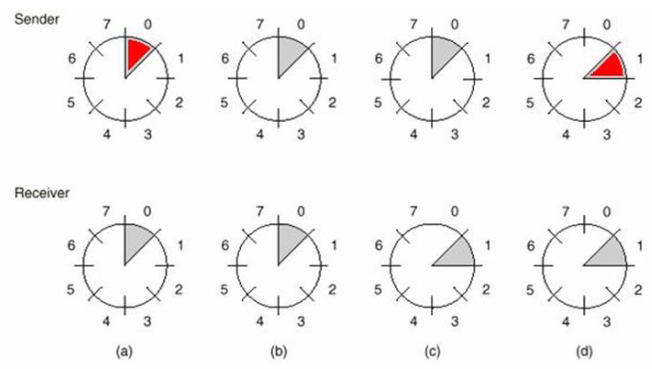
\includegraphics[width=0.42\textwidth]{pic/CN3/Sliding Window Protocols}
    \caption{A sliding window of size 1, with a 3-bit sequence number: (a) Initially. (b) After the first frame has been sent. (c) After the first frame has been received. (d) After the first acknowledgement has been received.}
\end{figure}

\subsubsection{One-Bit Sliding Window Protocol}%TODO 回去看代码, P88-
\begin{figure}[!htb]
    \centering
    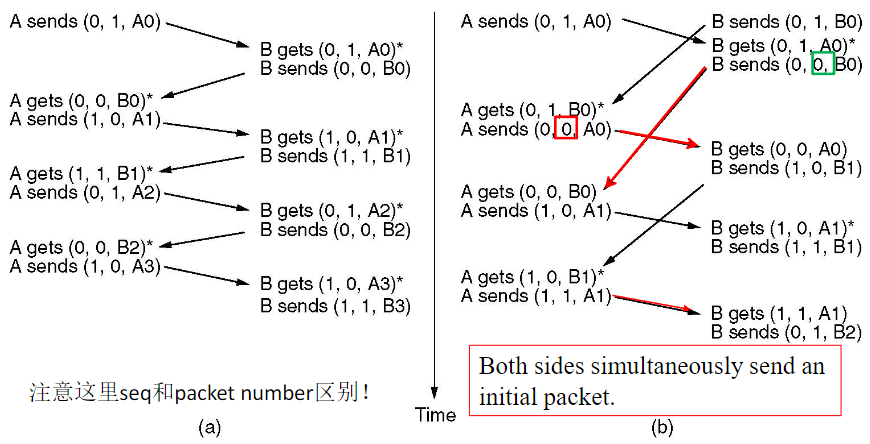
\includegraphics[width=0.42\textwidth]{pic/CN3/One-Bit Sliding Window Protocol}
    \caption{Two scenarios for protocol 4 (One-bit Sliding Window). (a) Normal case. (b) Abnormal case. The notation is (seq, ack, packet number). An asterisk indicates where a network layer accepts a packet. (Here the red arrows denotes the retransmissions because of timeout)}
\end{figure}

e.g. The rule requiring a sender to wait for an acknowledgement before sending another frame, 导致 bandwidth 利用率极低. The protocol 4 is disastrous in terms of efficiency under the situation of a long transit time, high bandwidth, and short frame length.

To find an appropriate value for $w$
\begin{enumerate}%TODO P92
    \item the bandwidth-delay product
    \item We can divide this quantity by the number of bits in a frame to express it as a number of frames. --- $BD$
    \item $w$ should be set to $2BD+1$
\end{enumerate}

\subsubsection{A Protocol Using Go Back N}
Pipelining frames over an unreliable channel raises some serious problem.
\begin{itemize}
    \item What happens if a frame in the middle of a long stream is damaged or lost?
    \item What should the receiver do with all the correct frames following a damaged frame?
\end{itemize}
Remember that the receiving data link layer is obligated to hand packets to the network layer in sequence.

\begin{figure}[!htb]
    \centering
    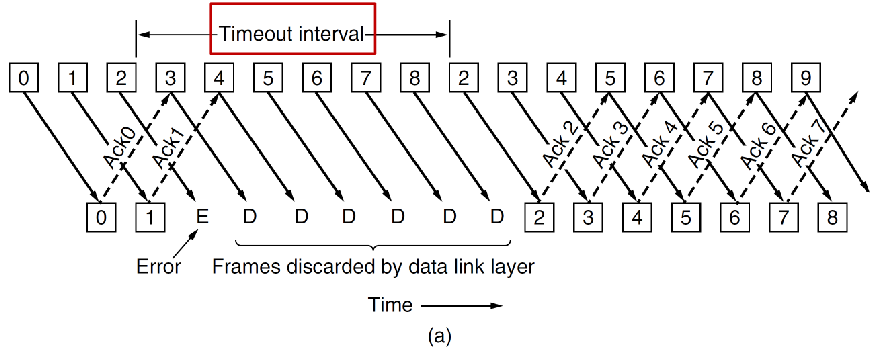
\includegraphics[width=0.42\textwidth]{pic/CN3/Receiver's window size is 1.}
    \caption{(a) Receiver's window size is 1. --- Go Back N}
    \label{fig:Go Back N}
\end{figure}
In \textbf{Figure} \ref{fig:Go Back N}, the receiver simply discard all subsequent frames, sending no acknowledgements for the discarded frames.

\begin{figure}[!htb]
    \centering
    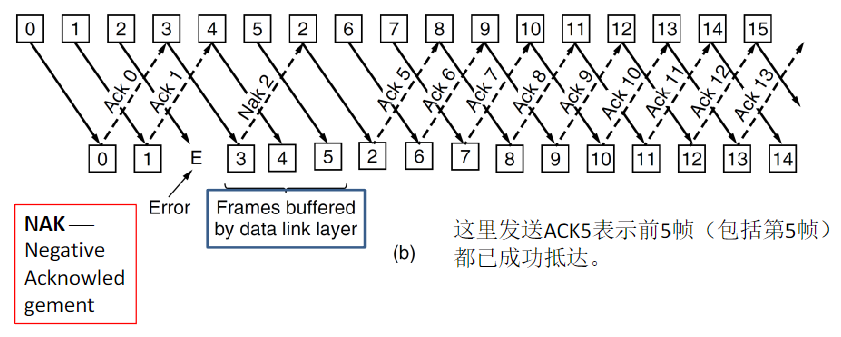
\includegraphics[width=0.42\textwidth]{pic/CN3/Receiver's window size is large.}
    \caption{Receiver's window size is large. --- Selective Repeat}
    \label{fig:Selective Repeat}
\end{figure}

In \textbf{Figure} \ref{fig:Selective Repeat}, a bad frame is received and discarded, but any good frames received after it are accepted and buffered. When the sender times out, only the oldest unacknowledged frame is retransmitted.

\paragraph{Assumptions}:
\begin{itemize}
    \item Data in both directions: piggybacking of ACK. (No separate ACK packets)
    \item Noisy channel
    \item Limited stream of data from network layer. (a ``network\_layer\_ready'' event)
\end{itemize}

\paragraph{Protocol}: Tanenbaum 5th edition: Fig. 3.19 %TODO 自己看 P97-

The sender window of size n. The receive window of size 1. 

%TODO P102-103 Normal Case, Damaged or Lost Case

$MAX\_SEQ$+1 distinct sequence numbers $(0, 1, 2, \dots, MAX\_SEQ)$, no more than $MAX\_SEQ$ unacknowledged frames, the sender $window\le MAX\_SEQ$. %TODO P104-105

\begin{figure}[!htb]
    \centering
    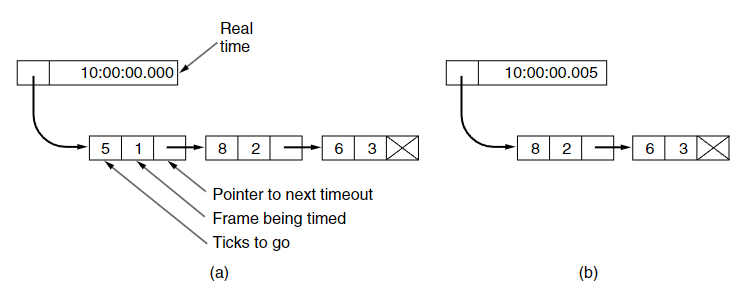
\includegraphics[width=0.42\textwidth]{pic/CN3/Simulation of multiple timers in software}
    \caption{Simulation of multiple timers in software.  (a) The queued timeouts. (b) The situation after the first timeout has expired.}
\end{figure}

\subsubsection{A Sliding Window Protocol Using Selective Repeat}
The selective repeat protocol is to allow the receiver to accept and buffer the frames following a damaged or lost one. 

\paragraph{Assumptions}: 
\begin{itemize}
    \item Data in both directions: piggybacking of ACK. (Separate ACK packets (requires ACK timer), accelerate ack)
    \item Noisy channel
    \item Limited stream of data from network layer
    \item NACK packets: receiver detected problem
\end{itemize}

\paragraph{Protocol}: Tanenbaum 5th Edition Fig. 3.21

%TODO P108-110 摸了
% \begin{enumerate}\small 
%     \item The sender’s window size starts out at 0 and grows to some
%     predefined maximum.
%     \item The receiver’s window, in contrast, is always fixed in size and
%     equal to the predetermined maximum.
%     \item The receiver has a buffer reserved for each sequence number within
%     its fixed window. Associated with each buffer is a bit (arrived) telling
%     whether the buffer is full or empty. Whenever a frame arrives, its
%     sequence number is checked by the function “between” to see if it
%     falls within the window. If so and if it has not already been received, it
%     is accepted and stored.
% \end{enumerate}
Nonsequential receive introduces further constraints on frame sequence number compared to protocols in which frames are only accepted in order!


%TODO e.g. P111-113

%TODO P114-117


\subsection{Examples of data link protocols}
point-to-point lines in the internet in two common situations:
\begin{itemize}
    \item SONET 
    \item ADSL (Asymmetric Digital Subscriber Loop)
\end{itemize}

\subsubsection{Point-to-Point Protocol}
A standard protocol called PPP (Point-to-Point Protocol) is used to send packets over these links.


PPP provides three main features:
\begin{enumerate}
    \item A framing method that unambiguously delineates the end of one frame and the
    start of the next one. The frame format also handles error detection.
    \item A link control protocol for bringing lines up, testing them, negotiating options,
    and bringing them down again gracefully when they are no longer needed. This
    protocol is called LCP (Link Control Protocol).
    \item A way to negotiate network-layer options in a way that is independent of the
    network layer protocol to be used. The method chosen is to have a different
    NCP (Network Control Protocol) for each network layer supported.
\end{enumerate}


\subsubsection{Packet over SONET}
SONET is the physical layer protocol. It provides a bitstream that runs at a well-defined rate. This bitstream is organized as fixed-size byte payloads that recur every 125 $\mu$sec, whether or not there is user data to send.

PPP runs on IP router to provide the transmission mechanism %TODO P123

The PPP frame format %TODO P123


\subsubsection{The PPP Frame Format}
All PPP frames begin with the standard HDLC flag byte of 0x7E (01111110).%TODO P124

\begin{itemize}
    \item The Address field
    \item The Control field
    \item The Protocol field
    \item The Payload field (1500 bytes)
    \item The Checksum field
\end{itemize}

\subsubsection{PPP Link Up \& Down}
%TODO P126

\subsubsection{ADSL (Asymmetric Digital Subscriber Loop)}
%TODO P128


An AAL5 frame %TODO P130

%TDOO 12:13 讲了作业 
    \newpage
\section{The Medium Access Control(MAC) Sublayer}
网络连接分两种: P2P or Broadcasting

MAC 是 Broadcasting. 

\subsection{The Channel Allocation Problem}
Static channel allocation: FDMA (bandwidth 分 $N$ 等大的块, 每个人一块)

但网络有 bursty (突发性), 所以使用 Dynamic channel allocation, also called Statistical Multiplexing. 


\subsubsection{Preliminary Queueing Theory}
\begin{align*}
    T_N=\frac{1}{\mu (C/N)-(\lambda/N)}=\frac{N}{\mu C-\lambda}=NT
\end{align*}
\begin{itemize}
    \item Consider any system that has a capacity $C$, the maximum rate at which it can perform work
    \item Assume that $R$ represents the average rate at which work is demanded from this system.
\end{itemize}

If $R<C$, 系统可以处理工作, 但因为有 the irregularity of the demands, 所以还是不行. If $R>C$, 系统寄. 

Two unpredictable sources lead to the irregularity of the demands:
\begin{enumerate}
    \item the arrival times
    \item the service times
\end{enumerate}


Queueing Theory: the characterization of the arrival times and the service times and the evaluation of their effect on queueing phenomena form the essence of queueing theory.

Let $C_n$ denote the $n$-th customer to arrive at a queueing facility, and 
\begin{itemize}
    \item $\tau_n=$ arrival time for $C_n$
    \item $t_n=\tau_n-\tau_{n-1}=$ interarrival time between $C_n$ and $C_{n-1}$
    \item $x_n=$ service time for $C_n$. 
\end{itemize}
$\{ t_n\}$,  $\{ \tau_n \}$ 是随机变量且独立分布. 定义两个一般随机变量:
\begin{itemize}
    \item $\tilde{t}=$ interarrival time
    \item $\tilde{x}=$ service time
\end{itemize}

probability distribution function (PDF)
\begin{itemize}
    \item $A(t)=P[\tilde{t}\le t]$
    \item $B(x)=P[\tilde{x}\le x]$
\end{itemize}

probability density function (pdf)
\begin{itemize}
    \item $a(t)=\frac{d A(t)}{dt}$
    \item $b(x)=\frac{d B(x)}{dx}$
\end{itemize}

important moments 联系这些随机变量
\begin{itemize}
    \item $E[\tilde{t}]=$ mean interarrival time $=\frac{1}{\lambda}$, where $\lambda$ is the average arrival rate. 
    \item $E[\tilde{x}]=$ mean service time $=\frac{1}{\mu}$. 
\end{itemize}

The study of queues naturally breaks into three cases:
\begin{enumerate}
    \item elementary queueing theory
    \item intermediate queueing theory
    \item advanced queueing theory
\end{enumerate}
根据 $a(t)$ 与 $b(x)$ 区分. 

A three-component description $A/B/m$, which denotes 
\begin{itemize}
    \item $m$-server queueing system
    \item $A$ the interarrival time distribution
    \item $B$ the service time distribution
\end{itemize}

And distributions symbols:
\begin{itemize}
    \item $M$ = exponential (i.e. Markovian)
    \item $Er$ = r-stage Erlangian
    \item $Hr$ = r-stage Hyperexponential
    \item $D$ = Deterministic
    \item $G$ = General
\end{itemize}

The simplest interesting system is the $M/M/1$ queue. 

\paragraph{General Results} The most important system parameter for $G/G/1$ is the utilization
factor $\rho$, 
\begin{align*}
    \rho=\lambda\tilde{x}
\end{align*}
单个 server 单位时间处于忙碌状态的时间. $\rho$ is the expected fraction of the system's capacity that is in use.

For multiple-server system $G/G/m$ 
\begin{align*}
    \rho=\frac{\lambda\tilde{x}}{m}
\end{align*}

In all cases a stable system is one for which $0\ge \rho<1$. 

The closer $\rho$ approaches unity, the larger are the queues and the waiting time.

The average time in system
\begin{align*}
    T=\tilde{x}+W
\end{align*}
where $W$ is waiting time in queue. 


\paragraph{Little's Result} 系统中平均客户数
\begin{align*}
    \bar{N}=\lambda T
\end{align*}

The average queue size is 
\begin{align*}
    \bar{N}_q=\lambda W
\end{align*}

In $G/G/m$, these quantities are related by
\begin{align*}
    \bar{N}_q=\bar{N}-m\rho
\end{align*}
可以理解为系统中平均客户数减去正在被服务的客户数就是正在等待服务的客户数了

动态客流:
\begin{itemize}
    \item $E_k$ $k$ customers 在系统中的状态
    \item $P_k(t)=P[N(t)=k]$ 在 $t$ 时, 系统处于 $E_k$ 的概率
    \begin{align*}
        \frac{dP_k(t)}{dt}=
    \end{align*}
\end{itemize}

Consider a stable system, $\displaystyle p_k=\lim_{t\to0} P_k(t)$. 

The $M/M/1$ queue: 
\begin{itemize}
    \item This system has a Poisson input. 
    \item The probability $P_k(t)$ of $k$ arrivals in an interval whose duration is $t$ sec is given by
    \begin{align*}
        P_k(t)=\frac{(\lambda t)^k}{k!}e^{-\lambda t}
    \end{align*}
    \item The average number of arrivals during this interval is
    \begin{align*}%TOOD 15
        \bar{N}(t)=\sum_{k=0}^{\infty} kP_k(t)=\lambda t
    \end{align*}
    So the average arrival rate in a unit time is $\lambda$.
    \item The average service time is $\tilde{x}=\frac{1}{\mu}$
    \item The probability of having $k$ customers in the system is given by
    \begin{align*}
        p_k=(1-\rho)\rho^k
    \end{align*}
    \item The average number in the system is
    \begin{align*}
        \bar{N}=\sum_{k=0}^\infty kp_k=\frac{\rho}{1-\rho}
    \end{align*}
    \item Using Little's result and the average time in the system $T$ is
    \begin{align*}
        T=\frac{\bar{N}}{\lambda}=\frac{\frac{1}{\mu}}{1-\rho}
    \end{align*}
    \item $W$ is
    \begin{align*}
        W&=\frac{\bar N_q}{\lambda}=\frac{\frac{\rho}{\mu}}{1-\rho}\\
        \bar N_q&=\bar N -m\rho =\frac{\rho^2}{1-\rho}
    \end{align*}
\end{itemize}

\subsubsection{The Performance of Static FDM}
The mean time delay $T$ to send a frame onto a channel of capacity $C$ bps (Note only one channel here). Assume
\begin{itemize}
    \item the average arrival rate $\lambda$
    \item the average length  $\frac{1}{\mu}$
    \item the service rate $\tilde{x}=\frac{1}{\mu C}$
    \item The utilization factor $\rho=\lambda\tilde{x}$
    \item According to the results of the $M/M/1$ queue
    \begin{align*}
        T=\frac{\frac{1}{\mu C}}{1-\rho}=\frac{1}{\mu C-\lambda}
    \end{align*}
\end{itemize}

Let us divide the single channel into $N$ independent subchannels, each with capacity $C/N$ bps. For subchannels:
\begin{itemize}
    \item mean input rate $\frac{\lambda}{N}$
    \item According to the results of an $M/M/m$ queue, the mean time delay
    \begin{align*}
        T_N=\frac{1}{\mu(C/N)-(\lambda /N)}=\frac{N}{\mu C-\lambda}=NT
    \end{align*}
\end{itemize}
分别排队等待时间更长. 

\subsubsection{Key Assumptions of Dynamic Channel Allocation}
Five key assumptions:
\begin{enumerate}\small
    \item Independent Traffic: The model consists of N independent stations. 每个人收发信号随机且独立. 
    \item Single Channel: A single channel is available. 所以可能有冲突. 
    \item Observable Collisions: All stations can detect the collision when it occurred. 
    \item Continuous or Slotted Time: Frame transmission can begin at any instant, or must begin at the start of a slot. (连续 or 有时钟)
    \item Carrier Sense or No Carrier Sense: (发送前是否检测信道状态) 
    \subitem With the carrier sense assumption, stations can tell if the channel is in use before trying to use it.
    \subitem If there is no carrier sense, stations cannot sense the channel before trying to use it. 
\end{enumerate}

\subsection{Multiple Access Protocols}
\subsubsection{ALOHA}
Each user terminal sharing the same upstream frequency to send frames to the central computer.

Two versions of ALOHA: pure and slotted.

\subsubsection{Pure ALOHA}
sender 向 central computer 发 frame, 然后 central computer rebroadcasts the frame to all of the stations, sender 监听这个转播来确定是否发送成功. (收到的frame 需要 和 发送的一致) 如果发送失败, sender 等待随机时间后再次发送. 

\begin{figure}[!htb]
    \centering
    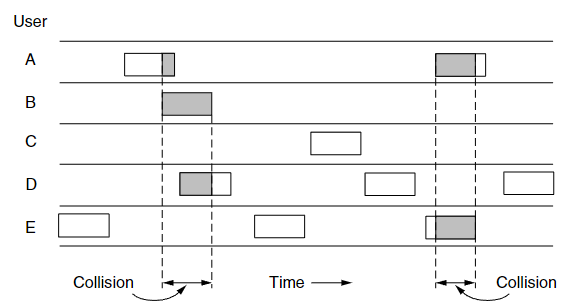
\includegraphics[width=0.309\textwidth]{pic/CN4/pure ALOHA.png}
    \caption{In pure ALOHA, frames are transmitted at completely arbitrary times.}
\end{figure}
If the first bit of a new frame overlaps with just the last bit of a frame that has almost finished, both frames will be totally destroyed.

An interesting question is: what is the efficiency of an ALOHA channel?
\begin{itemize}
    \item a Poisson distribution
    \item with mean of $N$ new frames per frame time. % (ppt) 中是 N
    \subitem If $N>1$, 超过信道容量, 寄. 
    \subitem expect $0<N<1$ 
    \item with mean of $G$ old frames per frame time.
    \subitem $G\ge N$
    \subitem At load low ($N\approx 0$), $G\approx N$
    \subitem At high low, $G>N$
    \subitem the throughput $S=GP_0$,  $P_0$ is the probabilityof a transmission succeeding

    \begin{figure}[!htb]
        \centering
        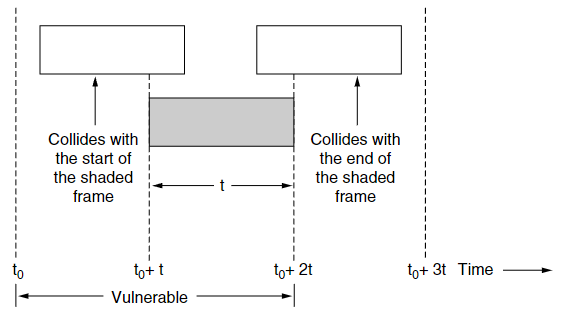
\includegraphics[width=0.309\textwidth]{pic/CN4/Vulnerable period for the shaded frame}
        \caption{Vulnerable period for the shaded frame}
    \end{figure}
    对一帧要保证 $2t$ 时间内没有其他帧发送. 
    \item The probability that $k$ frames are generated during a given frame time
    \begin{align*}
        P[k]=\frac{G^ke^{-G}}{k!},\ G\sim \lambda t
    \end{align*}
    \subitem The probability of zero frames is $e^{-G}$
    \subitem the entire vulnerable period is $P_0=e^{-2G}$
\end{itemize}

\begin{figure}[!htb]
    \centering
    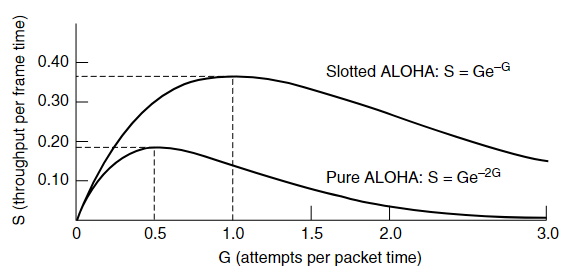
\includegraphics[width=0.309\textwidth]{pic/CN4/Throughput versus offered traffic for ALOHA systems.}
    \caption{Throughput versus offered traffic for ALOHA systems.}
\end{figure}
pure ALOHA 的最值在 $G=0.5$ 处.  Slotted ALOHA 的在 $G=1$ 处. 

\subsubsection{Slotted ALOHA}
divide time into discrete intervals called slots, agree on slot boundaries: 帧只能在 slot 的起点发. 

The probability of no other traffic is $e^{-G}$, so $S=Ge^{-G}$. The probability of a collision is  $1-e^{-G}$. 

推导:
\begin{itemize}
    \item The probability of a transmission requiring exactly $k$ attempts is
    \begin{align*}
        P_k=e^{-G}(1-e^{-G})^{k-1}
    \end{align*}
    \item The expected number of transmissions $E$ is
    \begin{align*}
        E=\sum_{k=1}^\infty kP_k=e^G
    \end{align*}
\end{itemize}
As a result of the exponential dependence of $E$ upon $G$, small increases in the channel load can drastically reduce its performance.

\subsubsection{Carrier Sense Multiple Access(CSMA) Protocols}
With slotted ALOHA, the best channel utilization that can be achieved is $1/e$. 因为任意发送太容易导致冲突了. 

\paragraph{1-persistent CSMA} 先监听信道看是否空闲, 空闲就发送, 不空闲一直侦听直到信道空闲然后发送. 遇到冲突仍然是等待随机时间再执行. The protocol is called 1-persistent because the station transmits with a probability of 1 when it finds the channel idle. 

\paragraph{Nonpersistent CSMA} 先监听信道看是否空闲, 空闲就发送, 不空闲等待随机时间然后再重复算法. 

\paragraph{p-persistent CSMA} applies to slotted channels. 先监听信道看是否空闲,空闲有 $p$ 概率发送, $1-p$ 概率不发送, 等待下一个slot. 不空闲就等待下一个 slot 

\begin{figure}[!htb]
    \centering
    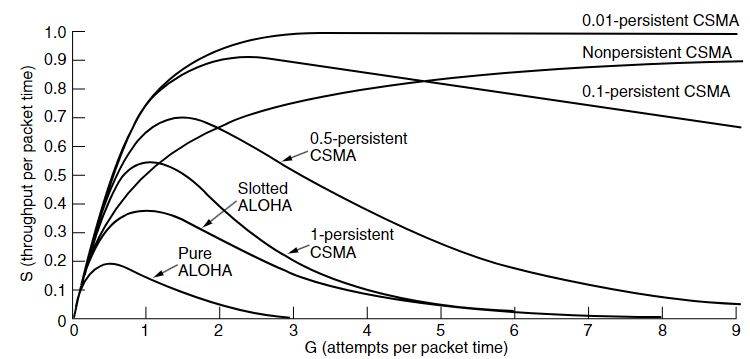
\includegraphics[width=0.309\textwidth]{pic/CN4/Comparison of the channel utilization}
    \caption{Comparison of the channel utilization versus load for various random access protocols.}
\end{figure}


\subsubsection{CSMA with Collision Detection}
Collision detection 边发送边读取. 若读的数据与发的一样就继续, 否则就是产生冲突, 中止发送. 

\begin{figure}[!htb]
    \centering
    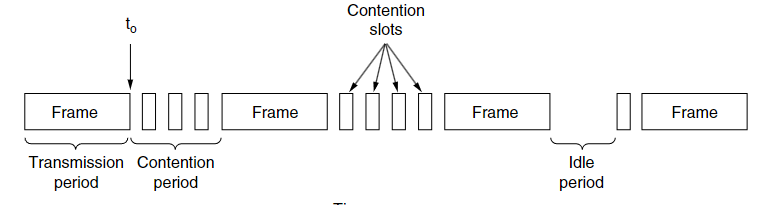
\includegraphics[width=0.42\textwidth]{pic/CN4/CSMA CD}
    \caption{CSMA/CD can be in contention, transmission, or idle state}
\end{figure}

Suppose that two stations both begin transmitting at exactly time $t_0$. How long will it take them to realize that they have collided?
\begin{itemize}
    \item Consider the worst-case scenario. propagate between the two farthest stations is $\tau$
    \item 在 $t_0$ A 发送, 在 $t_0 + \tau -\epsilon$ 时 B 发送, 直到 $2\tau-\epsilon$ 冲突才被 A 探测. 
\end{itemize}
We can think of CSMA/CD contention as a slotted ALOHA system with a slot width of $2\tau$.  

\subsubsection{Collision Free Protocols}
若 the bandwidth-delay product 大, 冲突影响大. 所以来些 没有冲突的算法. 

\paragraph{A Bit-Map Protocol --- Reservation Protocol} $N$ slots, 当作 bit map, bit 1 是发, 仅一个 1 时才发. 但不支持过大的网络. 
\begin{figure}[!htb]
    \centering
    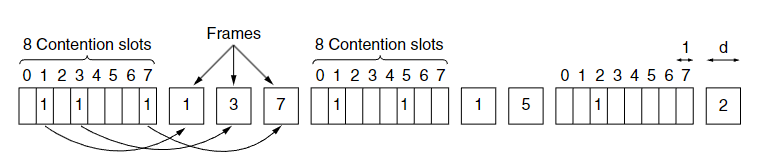
\includegraphics[width=0.42\textwidth]{pic/CN4/The basic bit-map protocol}
    \caption{The basic bit-map protocol}
\end{figure}

\paragraph{Token Passing}令牌轮询, 只有拿到令牌才能发送数据. 但令牌产生与销毁会导致不公平. 
\begin{figure}[!htb]
    \centering
    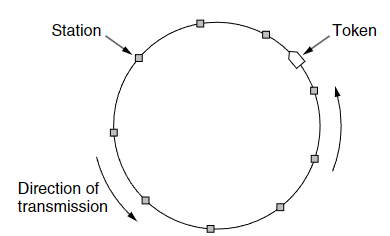
\includegraphics[width=0.309\textwidth]{pic/CN4/Token ring}
    \caption{Token ring}
\end{figure}

\paragraph{Binary Countdown}结合前两方法的优点. 每个站点给个编号, 更大的站点发. 

\subsubsection{Limited-Contention Protocols}
Two important performance measures broadcast network:
\begin{itemize}
    \item delay at low load
    \item channel efficiency at high load.
\end{itemize}


Limited-contention Protocols combine the best properties of the contention and collision-free protocols.
\begin{itemize}
    \item 每个站点有 $p$ 概率获得信道
    \item 但一个站点获得信道, 其他所有站点有 $1-p$ 不获得信道. The value is $kp(1-p)^{k-1}$
\end{itemize}
when $p=\frac{1}{k}$, the value is max. 
\begin{align*}
    Pr[\text{success with optimal} p]=\left( \frac{k-1}{k} \right)^{k-1}
\end{align*}

\begin{figure}[!htb]
    \centering
    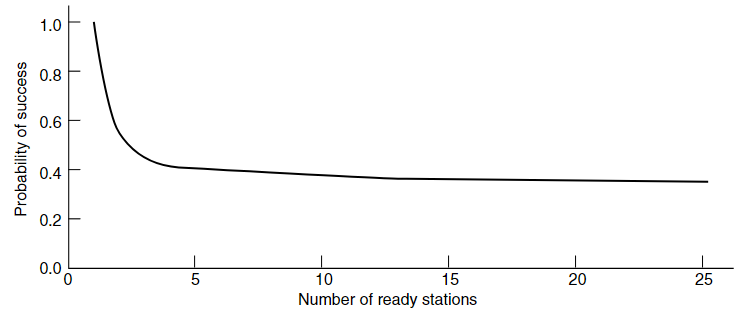
\includegraphics[width=0.42\textwidth]{pic/CN4/Acquisition probability for a symmetric contention channel}
    \caption{Acquisition probability for a symmetric contention channel}
\end{figure}
As soon as the number of stations reaches 5, the probability has dropped close to its asymptotic value of $1/e$.

所以将用户分组, group $x$ 竞争 slot $x$, 成功发送, 失败不发. 合适分组可以降低竞争程度. low load with big group, high load with small group. 


\paragraph{The Adaptive Tree Walk Protocol}结点1 是所有用户, 冲突后会分结点, 进行DFS, 成功会进行 BFS. 
\begin{figure}[!htb]
    \centering
    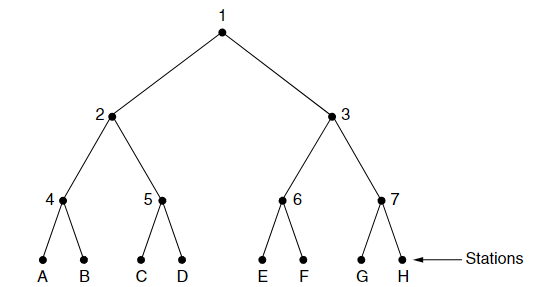
\includegraphics[width=0.309\textwidth]{pic/CN4/The tree for eight stations}
    \caption{The tree for eight stations}
\end{figure}


\subsubsection{Wireless LAN Protocols}
Wireless is more complicated than the wired case
\begin{itemize}
    \item Nodes may have different coverage areas. 
    \subitem 不同结点覆盖区域不同, 要避免之间的冲突. 
    \begin{figure}[!htb]
        \centering
        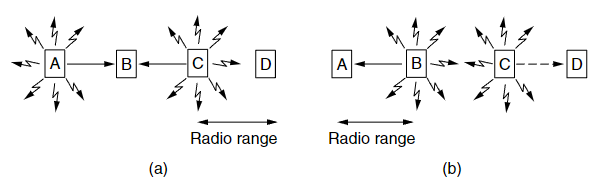
\includegraphics[width=0.42\textwidth]{pic/CN4/A wireless LAN.}
        \caption{A wireless LAN. (a) A and C are \textbf{hidden terminals} when transmitting to B. (b) B and C are \textbf{exposed terminals} when transmitting to A and D.}
    \end{figure}
    \item Nodes cannot hear while sending
    \subitem A node can hardly hear anything while sending messages. 
\end{itemize}

\paragraph{Possible Solution: MACA} (Multiple Access with Collision Avoidance) A short handshake before sending a frame

Protocol rules:
\begin{enumerate}
    \item A sender node transmits a RTS (Request-To-Send, with frame length)
    \item The receiver replies with a CTS (Clear-To-Send, with frame length)
    \item Sender transmits the frame while nodes hearing the CTS stay silent
\end{enumerate}

\begin{figure}[!htb]
    \centering
    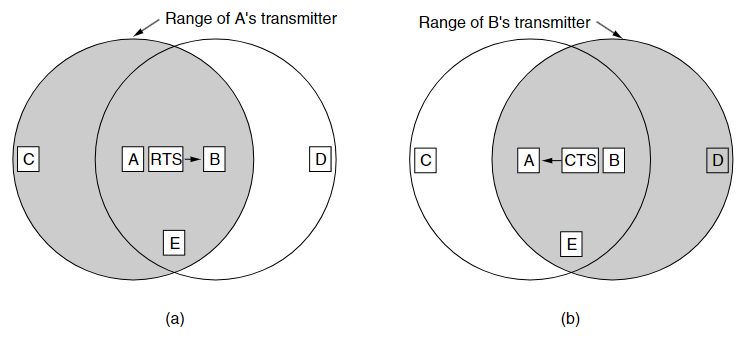
\includegraphics[width=0.309\textwidth]{pic/CN4/The MACA protocol.}
    \caption{The MACA protocol. (a) A sending an RTS to B. (b) B responding with a CTS to A.}
\end{figure}
\begin{itemize}
    \item 任意收到 RTS 的站点需要等待一个时间来保证 A 接受了 CTS. 
    \item 任意收到 CTS 的站点需要保持静默直到数据传输完成, 静默时间可以由CTS中信息决定. 
\end{itemize}

\subsection{Ethernet(IEEE 802.3)}
Two kinds of Ethernet exist
\begin{itemize}
    \item Classical Ethernet: 3 to 10 Mbps
    \item Switched Ethernet: runs at 100, 1000 and 10,000 Mbps
\end{itemize}
Over the cables, information was sent using \textbf{the Manchester encoding}.
\begin{figure}[!htb]
    \centering
    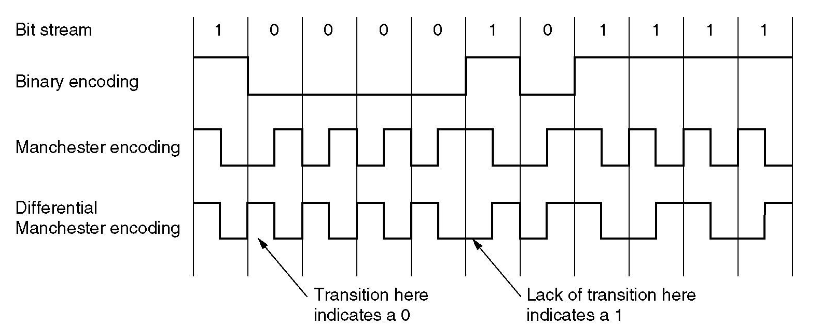
\includegraphics[width=0.42\textwidth]{pic/CN4/the Manchester encoding}
    \caption{the Manchester encoding}
\end{figure}

Ethernet brief history:
\begin{enumerate}
    \item In the mid-1970s, a bus topology. (A broadcast LAN)
    \item By the late 1990s, a hub-based star topology. A hub is a physical layer device. (A broadcast LAN)
    \item In the early 2000s, a switch --- a switch-based star topology (switched Ethernet). A switch is a link layer device. Modern switches are full-duplex. In a switch-base Ethernet LAN there are no collisions. 
\end{enumerate}


Ethernet is by far the most prevalent wired LAN technology. All of the Ethernet technologies provide \textbf{connectionless service} to the network layer.

\subsubsection{Ethernet Frame Structure}
\begin{figure}[!htb]
    \centering
    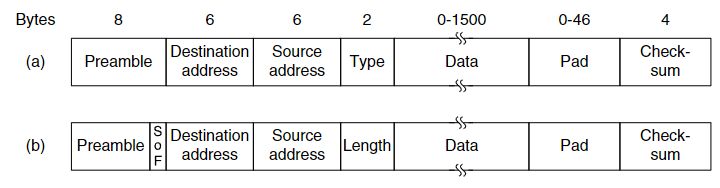
\includegraphics[width=0.42\textwidth]{pic/CN4/Frame formats}
    \caption{Ethernet Frame formats. (a) Ethernet (DIX). (b) IEEE 802.3.}
\end{figure}
\begin{itemize}
    \item \textbf{Preamble}: 8 bytes, each containing the bit pattern
    10101010 (In 802.3, is 10101011). The last byte is called \textbf{the Start of Frame} delimiter for 802.3. It produces a 10-MHz square
    wave, allow the receiver's clock to \textbf{synchronize}. 
    \item \textbf{Two addresses} (MAC addresses): 6*2 bytes. 
    \subitem The first transmitted bit of the destination address is a 0 for ordinary addresses and a 1 for group addresses. 
    \subitem The special address consisting of all 1 bits is reserved for broadcasting. 
    \subitem The 48-bit number of source address. The first 3 bytes of the address field are assigned by IEEE(IEEE 给网卡制造商分配的). The last 3 bytes of the address and programs the complete address into the NIC(网卡制造商烧录进网卡的 id).
    \item The \textbf{Type or Length} field: 2 bytes
    \subitem Any number there less than or equal to 0x600 (1536) can be interpreted as Length, and any number greater than 0x600 can be
    interpreted as Type. 
    \subitem a type code of 0x0800 means that the data contains an IPv4 packet.
    \item The Data field: 46 to 1500 bytes. 
    \subitem This field carries the IP datagram. The maximum transmission unit (MTU) of Ethernet is 1500 bytes. 
    \subitem The minimum size of the data is 46 bytes. Ethernet 要求 from destination address to checksum 的 valid frame 长度必须至少为64 bytes. 
    \begin{figure}[!htb]
        \centering
        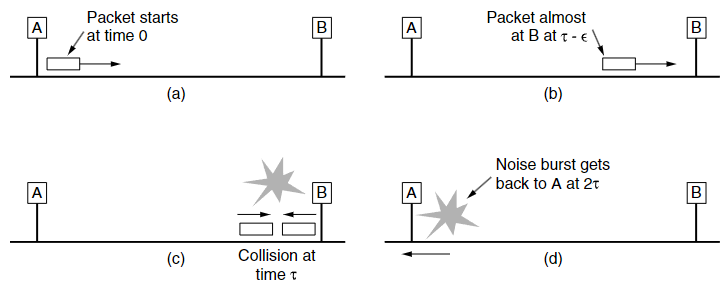
\includegraphics[width=0.42\textwidth]{pic/CN4/Collision detection}
        \caption{Collision detection can take as long as $2\tau$}
    \end{figure}
    \item \textbf{Checksum}: a 32-bit CRC
\end{itemize}

\subsubsection{CSMA/CD with Binary Exponential Backoff}
Classic Ethernet uses the 1-persistent CSMA/CD algorithm. 

How the random interval is determined when a collision occurs?%TODO 重点, 例子 P67
\begin{enumerate}
    \item After a collision
    \item After $i$ collision
    \item After $10$ collision
    \item After $16$ collision, the controller \textit{throws in the towel}(不干了) and reports failure back to the computer. 
\end{enumerate}

\subsubsection{Ethernet Performance}
Ethernet under conditions of heavy and constant load with $k$ stations always ready to transmit.

If each station transmits during a contention slot with probability $p$, the probability $A$ that some station acquires the channel in that slot is 
\begin{align*}
    A=kp(1-p)^{k-1}
\end{align*}
$A$ is maximized when $p=\frac{1}{k}$, with $A\to \frac{1}{e}$ as $k\to\infty$. 

The probability that the contention interval has exactly $j$ slots in it is $A(1-A)^{j-1}$, so the mean number of slots per contention is given by
\begin{align*}
    \sum_{j=0}^\infty jA(1-A)^{j-1}=\frac{1}{A}
\end{align*}
%TODO P69 是上述两式的具体推导. 

Since each slot has a duration $2\tau$, the mean contention interval $w=\frac{2\tau}{A}$. 

If the mean frame takes $P$ sec to transmit,  transmit, when many stations have frames to send
\begin{align*}
    \text{Channel efficiency}=\frac{P}{P+\frac{2\tau}{A}}
\end{align*}
The longer the cable, the longer the contention interval. 

In terms of the frame length, F, the network bandwidth, B, the cable length, L, and the speed of signal propagation, c, for the optimal case of e contention slots per frame. With $P=\frac{F}{B}$, 
\begin{align*}
    \text{Channel efficiency}=\frac{1}{1+\frac{2BLe}{cF}}
\end{align*}
\begin{figure}[!htb]
    \centering
    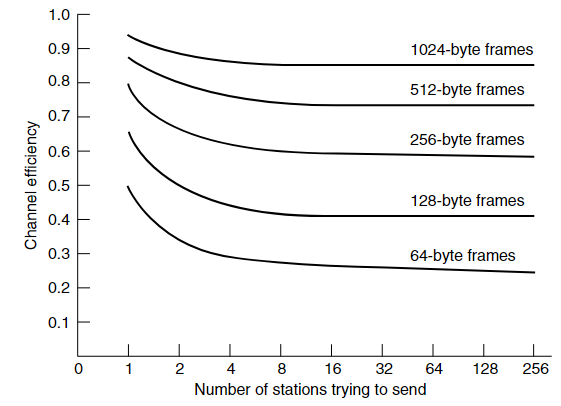
\includegraphics[width=0.309\textwidth]{pic/CN4/Efficiency of Ethernet}
    \caption{Efficiency of Ethernet at 10 Mbps with 512-bit slot times.}
\end{figure}%TODO 修 P -71

\subsubsection{Switched Ethernet}
\begin{figure}[!htb]
    \centering
    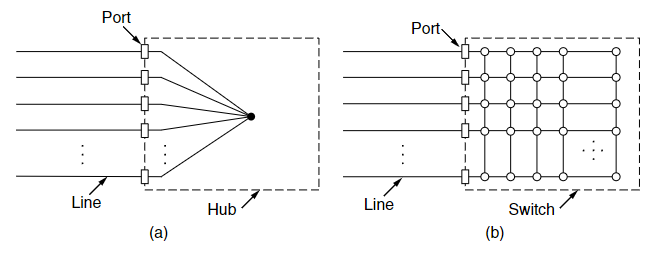
\includegraphics[width=0.42\textwidth]{pic/CN4/Hub and Switch}
    \caption{ (a) Hub. (b) Switch.}
\end{figure}

In a hub, all stations are in the same collision domain. But in a switch, each port is its own independent collision domain.
\begin{figure}[!htb]
    \centering
    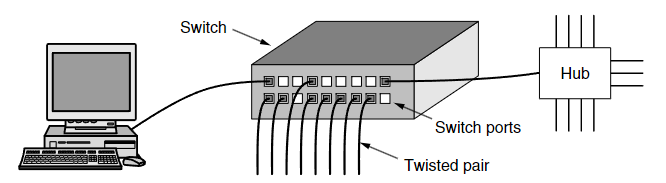
\includegraphics[width=0.42\textwidth]{pic/CN4/An Ethernet switch}
    \caption{An Ethernet switch}
\end{figure}

\subsubsection{Ethernet Technologies}
There are many other Ethernet technologies have been standardized over the years by the IEEE 802.3 CSMA/CD (Ethernet) working group.

e.g. 10BASE-T, 10BASE-2, 100BASE-T, 1000BASE-LX and 10GBASE-T. 

Ethernet is both a link-layer and a physical-layer specification. 

\subsubsection{Gigabit Ethernet}
All configurations of gigabit Ethernet use point-to-point links. 

supports two different modes of operation: 
\begin{itemize}
    \item full-duplex mode: there is a central switch connected to computers. 
    \item half-duplex mode: the computers are connected to a hub
    \subitem Carrier extension: at least 512 bytes
    \subitem Frame bursting
\end{itemize}

\subsection{Wireless LANS (802.11 WiFi)}
802.11 networks can be used in two modes
\begin{itemize}
    \item In infrastructure mode, each client is associated with an AP (Access Point), and APs may be connected together by a wired network
    \item Ad hoc network, there is no access point, and each computer can sent frames to each other directly.
\end{itemize}
\begin{figure}[!htb]
    \centering
    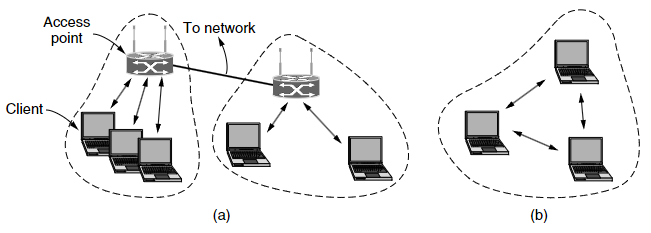
\includegraphics[width=0.42\textwidth]{pic/CN4/802.11 architecture}
    \caption{802.11 architecture. (a) Infrastructure mode. (b) Ad-hoc mode.}
\end{figure}

The data link layer in all the 802.11 protocols is split into two or more sublayers:
\begin{itemize}
    \item The MAC (Medium Access Control)
    \item The LLC (Logical Link Layer)
\end{itemize}
\begin{figure}[!htb]
    \centering
    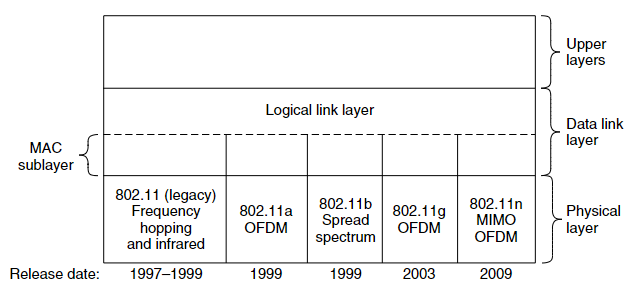
\includegraphics[width=0.42\textwidth]{pic/CN4/Part of the 802.11 protocol stack}
    \caption{Part of the 802.11 protocol stack}
\end{figure}

\subsubsection{802.11 Physical Layer}
Either the 2.4 GHz or the 5GHz ISM (Industrial, Scientific and Medical) frequency bands. 

%TODO 回顾专有名词/缩写

\subsubsection{The 802.11 MAC Sublayer Protocol}
Problems with wireless:
\begin{itemize}
    \item Half duplex: cannot transmit and listen for noise bursts at the same time on a single frequency
    \item Limited Range: The hidden station problem and the exposed station problem    
\end{itemize}
\begin{figure}[!htb]
    \centering
    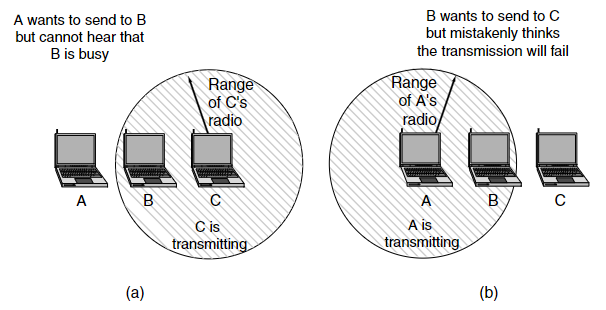
\includegraphics[width=0.42\textwidth]{pic/CN4/Problems with wireless}
    \caption{(a) The hidden terminal problem. (b) The exposed terminal problem.}
\end{figure}

The 802.11 tries to avoid collision with a protocol called CSMA/CA (CSMA with Collision Avoidance).
\begin{itemize}
    \item Channel sensing before sending
    \item Exponential backoff after collision
\end{itemize}
\begin{figure}[!htb]
    \centering
    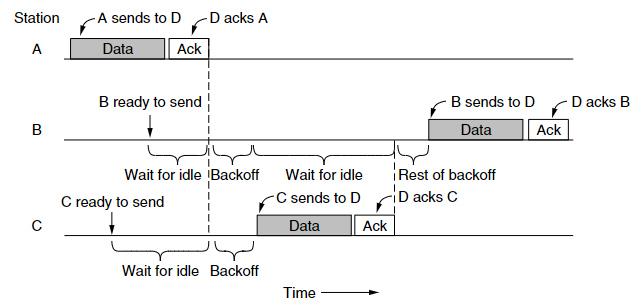
\includegraphics[width=0.42\textwidth]{pic/CN4/Sending a frame with CSMACA}
    \caption{Sending a frame with CSMA/CA. (A, B and C want to send frames to D.)}
\end{figure}


Compared to Ethernet, there are main two differences:
\begin{enumerate}
    \item starting backoffs early helps to avoid collision
    \item acknowledgements are used to infer collision( collision cannot be detected.)
\end{enumerate}

Two modes of operations (backoff):
\begin{enumerate}
    \item DCF (Distributed Coordination Function) because each station acts independently.
    \item PCF (Point Coordinate Function) in which the AP may act as the BS in the cellular network.
\end{enumerate}

To reduce ambiguities about which station is sending, 802.11 defines channel sensing to consists of physical sensing and virtual sensing.
\begin{enumerate}
    \item [Method 1] Physical sensing
    \begin{itemize}
        \item  If idle, just starts transmitting. Does not sense channel while transmitting.
        \item If collision occurs, wait random time, using Ethernet binary exponential backoff algorithm    
    \end{itemize}
    Be used to transmit RTS frame.
    \item [Method 2] Virtual Sensing
    \subitem Scenario: A wants to send to B. C is a station within range of A. D is a station within range of B but not within range of A. (C A B D)
    \begin{figure}[!htb]
        \centering
        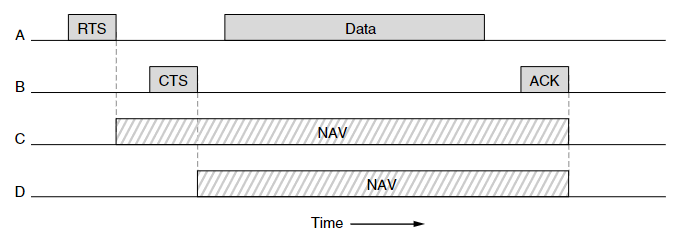
\includegraphics[width=0.42\textwidth]{pic/CN4/Virtual channel sensing using CSMACA}
        \caption{Virtual channel sensing using CSMA/CA}
    \end{figure}

    Note: the NAV signals are NOT transmitted; they are just internal reminder to keep quiet for a certain period of time.
\end{enumerate}

There are several other mechanisms to improve its performance:
\begin{enumerate}
    \item Reliability
    \subitem To lower the transmission rate. send shorter frames, allow frames to be split into smaller pieces, called fragments. 
    \item Power: the basic mechanism for saving power builds on beacon frames
    \item Quality of Services: After a frame has been sent, a certain amount of idle time is required before any station may send a frame to check that the channel is no longer in use. 
\end{enumerate}

\subsubsection{The 802.11 Frame Structure}
The 802.11 standard defines three different classes of frames in the air: data, control, and management. 
\begin{figure}[!htb]
    \centering
    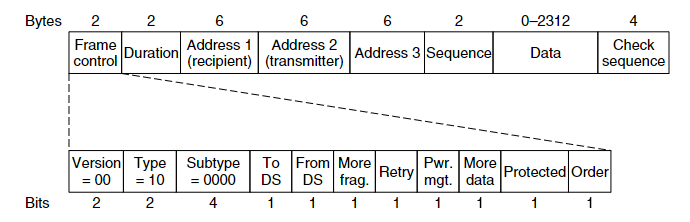
\includegraphics[width=0.42\textwidth]{pic/CN4/Format of the 802.11 data frame}
    \caption{Format of the 802.11 data frame}
\end{figure}

\begin{itemize}
    \item data frame
    \begin{itemize}
        \item Address fields: data frames sent to or from an AP, but the AP may be a relay point, so the Address 3 gives a distant destination.
        \item Protocol Version: set to 00
        \item Type: data, control, or management; Subtype: RTS, CTS, or ACK of control frame; for a regular data frame (without quality of service), they are set to 10 and 0000 in binary.
        \item To DS and From DS: to indicate whether the fame is going to or coming from the networks connected to the APs.
        \item More Fragments: more fragments will follow;
        \item Retry: retransmission;
        \item Pwr: sleep state;
        \item More data: sender has additional frames;
        \item The Protected Frame bit: encrypted usign WEP;
        \item The Order bit: processed strictly in order;
        \item Duration: time the frame and its acknowledgement takes; it also exists in control frame.
        \item Sequence: 16 bits, 12 for frame, 4 for fragment.
    \end{itemize}
    \item Management frames: similar to data frames, except without one of the base station addresses, because management frames are restricted to a single cell.
    \item Control frames: shorter
\end{itemize}

Each 802.11 LAN must provide nine services

\subsection{Data Link Layer Switching}
We can treat one physical LAN as multiple logical LANs, called
VLANs (Virtual LANs)

\subsubsection{Learning Bridge}%TODO 之后摸了 P101
All of the stations attached to the same port on a bridge belong to the same collision domain. 

%TODO 补图

have a big (hash) table. This table can list each possible destination and which output port it belongs to.  use a flooding algorithm:
\begin{itemize}
    \item Every incoming frame for an unknown destination is output on all the ports to
    which the bridge is connected except the one it arrived on
    \item Once a destination is known, frames destined for it are put only on the proper port
\end{itemize}

By looking at the source addresses, they can tell which machines are accessible on which ports. 

But the network topology is dynamic. To handle it, the arrival time of the frame is noted in the entry. 

Periodically, a process in the bridge scans the hash table and purges all entries more than a few minutes old.

The routing:
\begin{enumerate}
    \item If the port for the destination address is the same as the source port, discard the frame.
    \item If the port for the destination address and the source port are different, forward the frame on to the destination port.
    \item If the destination port is unknown, use flooding and send the frame on all ports except the source port.
\end{enumerate}

\subsubsection{Protocol Processing at a Bridge}
In the general case, relays at a given layer can rewrite the headers for that layer.

%TODO 补图, P 106

e.g. %图 P107

\subsubsection{Spanning Tree Bridges}% P108-


\paragraph{Spanning Tree Algorithm}

% e.g. 跳过吧


\subsection{Repeaters, Hubs, Bridges, Switches, Routers, and Gateways}%TODO P119
The layer matters because different devices use different pieces of information to decide how to switch

\subsubsection{Repeaters and Hubs (Physical Layer)}

\subsubsection{Bridges and Switches (Data Link Layer)}

\subsubsection{Routers (Network Layer)}

\subsubsection{Gateways}

\subsubsection{Virtual LANs}
    \newpage
\section{Newwork Layer}
\subsection{Overview of network layer}

\subsubsection{Two Important Network Layer Functions}
The role of the network layer is to move packets from a sending host to a receiving host.

Each router has a forwarding (internal, routing) table. The forwarding table is indexed by either the destination address in the packet header or an indication of connection to which the packet belongs. 

\begin{enumerate}
    \item Forwarding (the main function of a router)
    \item Routing (to build the forwarding table for each router): via routing protocols
\end{enumerate}

The issues include the service provided to the transport layer and the internal design of the network.
\begin{figure}[!htb]
    \centering
    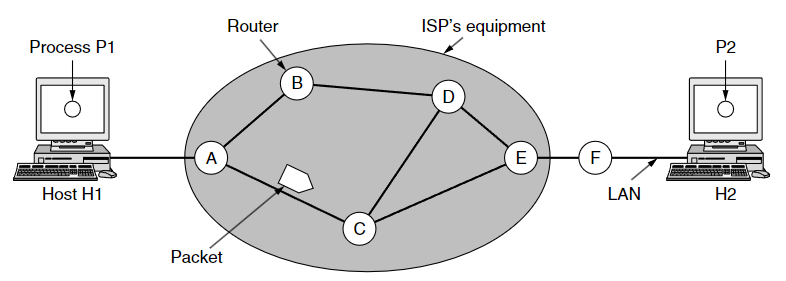
\includegraphics[width=0.309\textwidth]{pic/CN5/The environment of the network layer protocols}
    \caption{The environment of the network layer protocols}
\end{figure}

\subsubsection{Services Provided to the Transport Layer}
Design goals:
\begin{itemize}
    \item The services should be independent of the router technology
    \item The transport layer should be shielded from the number, type, and topology of the routers present
    \item The network addresses should use a uniform numbering plan.
\end{itemize}

Two warring factions, Connection-oriented \& Connectionless service. Network layer should provide connection-oriented service or connectionless service.

The packets are frequently called datagrams. 

\paragraph{Implementation of Connectionless Service}Packets are injected into the network individually and routed independently of each other. 

Every router has a forwarding table. Each table entry is a pair consisting of a destination and the outgoing line to use for that destination.

\begin{figure}[!htb]
    \centering
    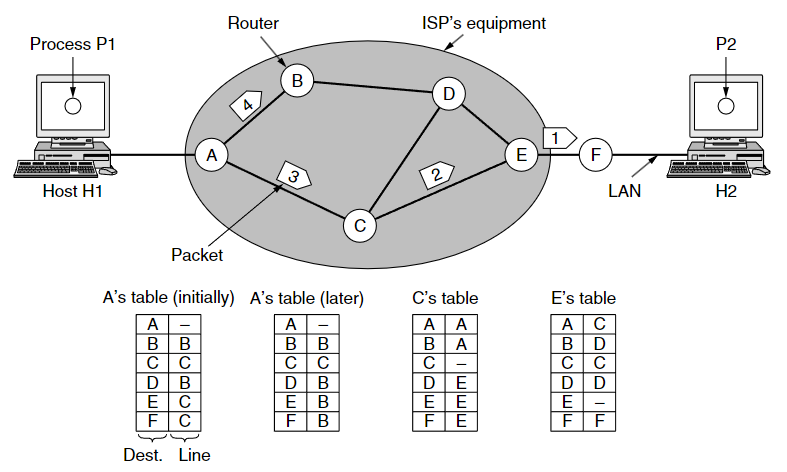
\includegraphics[width=0.309\textwidth]{pic/CN5/Routing within a datagram network}
    \caption{Routing within a datagram network}
\end{figure}


\paragraph{Implementation of Connection-Oriented Service}Each packet carries an identifier telling which virtual circuit it belongs to.

\begin{figure}[!htb]
    \centering
    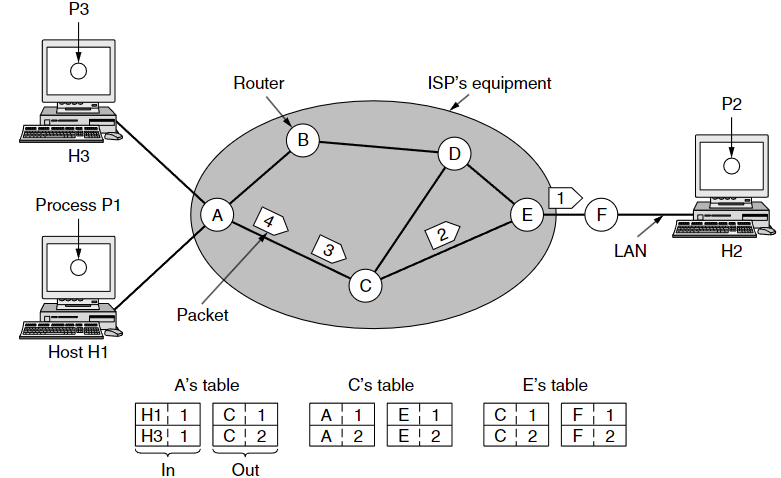
\includegraphics[width=0.309\textwidth]{pic/CN5/Routing within a virtual-circuit network}
    \caption{Routing within a virtual-circuit network}
\end{figure}


\begin{table}[!htb]%TODO P10
    \centering
    \caption{Virtual-Circuit vs. Datagram Networks}
    \begin{tabular}[c]{ccc}\toprule
         \\ \midrule
        
        \bottomrule
    \end{tabular}
\end{table}



\subsection{Routing algorithms}
Two functions of a router: 转发+建立路由表. 

Difference in Datagram and Virtual Circuit:
\begin{itemize}
    \item In datagram, route 实时更新
    \item In virtual circuit, route  仅在初始化时设定
\end{itemize}

\subsubsection{Classification of Routing Algorithms}
Classify routing algorithms into global routing algorithms and decentralized algorithms.
\begin{itemize}
    \item Global routing algorithms: 适用于小网络. e.g. Link-state (LS) algorithms
    \item Decentralized routing algorithms: 适用于大网络. e.g. Distance-vector (DV) algorithms
\end{itemize}

A second broad way to classify routing algorithm:
\begin{itemize}
    \item Static routing algorithms (non-adaptive)
    \item Dynamic routing algorithms (adaptive): 可能会摇摆, 有回路. 
\end{itemize}


\subsubsection{Link-state (LS) algorithms}
In a link-state algorithm, the network topology and all link costs
are known. 首先要 broadcast 以获得这些信息. 

All nodes have an identical and complete view of the network.

The well-known LS algorithm is Dijkstra's algorithm. 

\paragraph{The Shortest Path Algorithm}The shortest path is one that has the least cost. 

Measure path cost (length)
\begin{itemize}
    \item Number of hops
    \item Delay
    \item distance
    \item Bandwidth
    \item Communication cost
    \item Average traffic
\end{itemize}

The optimality principle: If router $J$ is on the optimal path from router $I$ to router $K$, then the optimal path from $J$ to $K$ also falls along the same route.

\paragraph{Sink Tree}
Sink tree for a destination is the union of all shortest paths towards the destination. Similarly source tree. 

Implications:
\begin{enumerate}
    \item Only need to use destination to follow shortest paths
    \item Each node only need to send to the next hop
\end{enumerate}

Forwarding table at a node List next hop for each destination. 

\paragraph{Dijkstra Algorithm}For single source shortest path problem. Approach: Greedy.

The Complexity of Dijkstra Algorithm: worst-case complexity is $O(n^2)$. 

\begin{figure}[!htb]
    \centering
    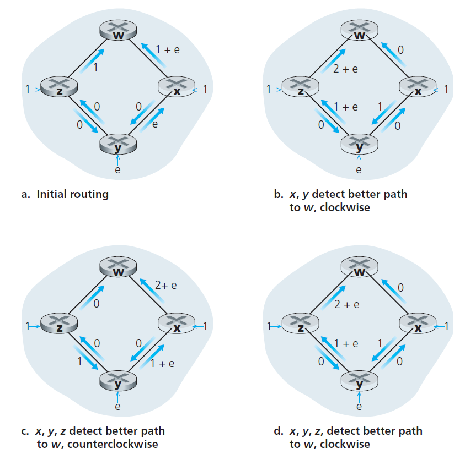
\includegraphics[width=0.309\textwidth]{pic/CN5/Oscillation}
    \caption{The Oscillation Problem with the LS Algorithm}
\end{figure}

\paragraph{Flooding(洪放)}Each router must make decisions based on local knowledge.In flooding, every incoming packet is sent out on every outgoing line except the one it arrived on. 但会有node 接收到重复的拷贝. 

e.g. Consider a flood from A: first reaches B via AB, E via AE. 

\begin{figure}[!htb]
    \centering
    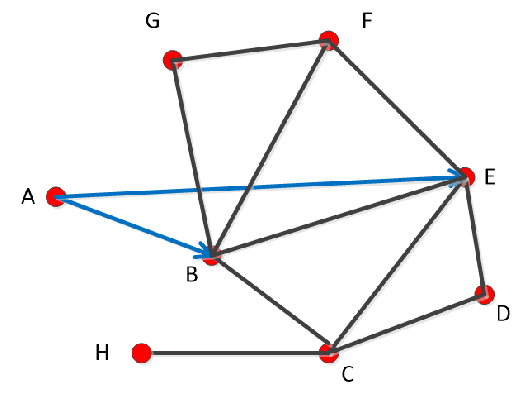
\includegraphics[width=0.309\textwidth]{pic/CN5/Flooding Example}
    \caption{Flooding Example}
\end{figure}

There are some solutions to avoid flooding duplicate packets.
\begin{enumerate}
    \item Solution 1: A hop counter contained in the header of each packet, packet is discarded when the counter reaches zero.
    \item Solution 2: Every node keeps track of which packets have been flooded, to avoid sending them out a second time.
\end{enumerate}

\paragraph{Link State Routing}:
\begin{enumerate}%TODO P45-50
    \item Learning about the neighbors
    \item Setting link costs
    \item Building link state packets
    \subitem The hard part is determining when to build them.
    \item Distributing the link state packets
    \subitem The fundamental idea is to use flooding to distribute the link state packets to all routers.
    \subitem The solution to all these problems is to include the age of each packet
    \subitem To guard against errors on the links, all link state packets are acknowledged.    
    \item Computing the new routes
\end{enumerate}

\subsubsection{Distance-vector (DV) algorithms}
The distance vector routing algorithm is iterative, asynchronous, and distributed. 
\begin{itemize}
    \item Distributed: 从邻居获取信息, 并给邻居信息. 
    \item Iterative: 迭代直到邻居没有信息变更. It is self-terminating. 
    \item Asynchronous: 不要求同步. 
\end{itemize}
DV-like algorithms are used in many routing protocols in practice, including the Internet's RIP, BGP, and so on.

\paragraph{Bellman-Ford Equation}
Let $d_x(y)$ be the cost of the least-cost path from node $x$ to node $y$. Then the least costs are related by the celebrated Bellman-Ford equation, namely,
\begin{align*}
    d_x(y)=\min_v\{ c(x,v)+d_d(y) \}
\end{align*}
where the $\min_v$ in the equation is taken over all of $x$'s neighbors.

\begin{figure}[!htb]
    \centering
    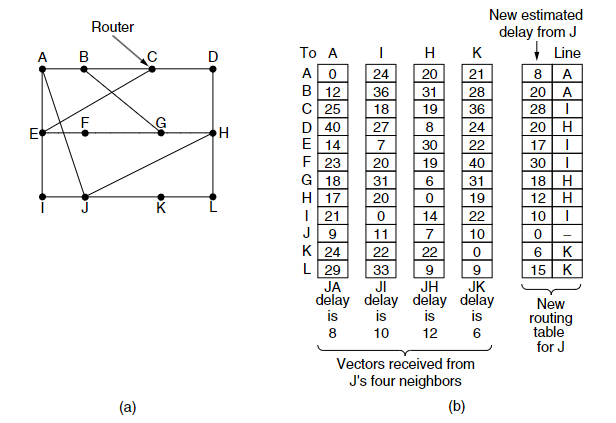
\includegraphics[width=0.309\textwidth]{pic/CN5/Bellman-Ford}
    \caption{(a) A network. (b) Input from $A, I, H, K$, and the new routing table for $J$}
\end{figure}

\paragraph{The Distance Vector Routing Algorithm}
The basic idea: each node $x$ begins with $D_x(y)$, an estimate of the cost of the least-cost path from itself to node $y$, for all nodes in $N$ (the number of nodes in the network). Let $D_x(y) = [D_x(y) : y \in N]$ be node $x$'s distance vector, which is the vector of cost estimates from $x$ to all other nodes, $y \in N$.

With the DV algorithm, each node $x$ maintains the following information:
\begin{itemize}
    \item $c(x, v)$: The cost, for each neighbor node $v$.
    \item $D_x(y)=[D_x(y):y\in N]$: Node $x$'s distance vector.
    \item $D_v(y)=[D_v(y):y\in N]$: The distance vectors of each of its neighbors.
\end{itemize}

\begin{enumerate}
    \item 接受新的 distance vector 后进行更新. 
    \item 有更新就广播给邻居
    \item 直到不变, $D_x(y)$ 收敛于 $d_x(y)$.
\end{enumerate}

最后达到 A quiescent state. 

\paragraph{The Count-to-Infinity Problem}
收敛可能所需时间过长. 

\begin{figure}[!htb]
    \centering
    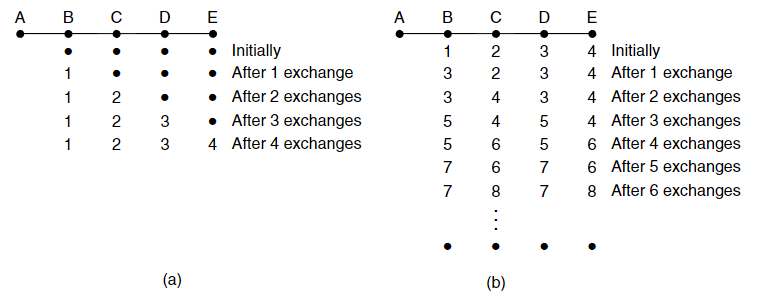
\includegraphics[width=0.42\textwidth]{pic/CN5/The count-to-infinity problem}
    \caption{The count-to-infinity problem}
\end{figure}
Suppose node A is down initially and all other routers know this. In other words, they have all recorded the delay to A as infinity.

\begin{table*}[!htb]
    \centering
    \caption{Distance Vector Routing vs. Link State Routing}
    \begin{tabular}[c]{c|cc}\toprule
        \multicolumn{1}{c}{\textbf{Goal}} & \textbf{Distance Vector} & \textbf{Link State} \\ \midrule
        Correctness & Distributed Bellman-Ford & Replicated Dijkstra's Algorithm \\
        Efficient Paths & Approx. with shortest paths & Approx. with shortest paths \\
        Fair Paths & Approx. with shortest paths & Approx. with shortest paths \\
        Convergence & Slow (many exchanges) & Fast (Flood and compute) \\
        Scalability & Excellent (storage/compute) & Moderate (storage/compute) \\
        \bottomrule
    \end{tabular}
\end{table*}


\subsubsection{Hierarchical Routing}the routers are divided into what we will call regions.

When routing is done hierarchically, there are entries for all the local routers, but all other regions are condensed into a single router.

\subsubsection{Broadcast Routing}the network layer provides a service of delivering a packet sent from a source node to all other nodes in the network. 
\begin{enumerate}
    \item One of the most simple and straightforward way is to send a separate copy of packet to each destination. 
    \item Multidestination routing: Each packet contains either a list of destinations or a bit map indicating the desired destinations
    \item Uncontrolled flooding %TODO 65-68
    \subitem the source node sends a copy of the packet to all of its neighbors
    \subitem Sequence-number-controlled flooding
    \subitem Reverse path forwarding (RPF)
    \item Spanning-Tree Broadcast
    \subitem core: the creation and maintenance of the spanning tree. The center-based approach to building a spanning tree:
    \begin{enumerate}
        \item A center node is defined.
        \item Nodes then unicast tree-join messages addressed to the center
        node. A tree-join message is forwarded using unicast routing
        toward the center until it either arrives at a node that already
        belongs to the spanning tree or arrives at the center.
        \item In either case, the path that the tree-join message has followed
        defines the branch of the spanning tree between the edge node that
        initiated the tree-join message and the center. Graft. 
    \end{enumerate}
\end{enumerate}

\subsubsection{Multicast Routing}%TODO P73-77 自己看

\subsubsection{Anycast Routing}
\begin{itemize}
    \item Unicast --- a single destination
    \item Broadcast --- to all destinations
    \item Multicast --- to a group of destinations
\end{itemize}
In anycast, a packet is delivered to the nearest member of a group. Anycast is used in the Internet as part of DNS. 


\subsection{The network layer in the Internet}
There are two basic choices for connecting different networks:
\begin{enumerate}
    \item build devices that translate or convert packets
    \item building a common layer on top of the different networks.
\end{enumerate}
IP is the foundation of the modern Internet. 

The network layer of the internet has three main components:
\begin{itemize}\small
    \item The IP protocol
    \item The Internet control protocols (including ICMP, DHCP, ARP)
    \item The Internet routing protocols (including RIP, OSPF and BGP)
\end{itemize}

\subsection{IP Protocol}
\subsubsection{The IPv4 Datagram}
The header has a 20-byte fixed part and a variable-length optional part. The bits are transmitted from left to right and top to bottom. This is ``big-endian'' network byte order.

\begin{figure}[!htb]
    \centering
    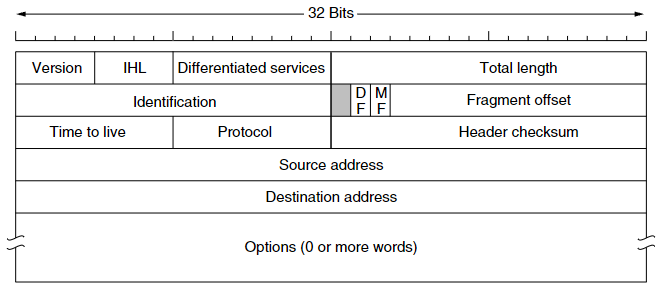
\includegraphics[width=0.42\textwidth]{pic/CN5/The IPv4 (Internet Protocol) header}
    \caption{The IPv4 (Internet Protocol) header}
\end{figure}
\begin{enumerate}
    \item The Version field (4 bits)
    \item IHL field (Header Length) (4 bits)
    \subitem tell how long the header is in 32-bit words, limits the
    header to 60 bytes, thus the options field to 40 bytes. 
    \subitem the typical IP datagram has a 20-bytes header.
    \item The Different Service field (Type of Service) (8 bits)
    \subitem The top 6 bits are used to mark the packet with its service class
    \subitem The bottom 2 bits are used to signal \textbf{explicit congestion indications}
    \item The Total Length field (16 bits)
    \subitem The total length of header and data.
    \subitem The theoretical maximum length is 65,535 bytes.
    \subitem Datagrams are rarely larger than 1,500 bytes. (由 以太网的 MTU 决定)
    \item The Identification field (16 bits), flags (DF, MF), and fragment offset (13 bits)
    \subitem All the fragments of a packet contain the same identification field.
    \begin{itemize}
        \item The Unused bit
        \item DF -- Don't Fragment
        \item MF -- More Fragments 
        \subitem (MF = 0 means this the last fragment)
        \item The Fragment Offset field (13 bits)
        \subitem There is a maximum of 8192 fragments per datagram
    \end{itemize}
    \item The TtL (Time to live) field (8 bit)
    \subitem This field is decremented by one each time the datagram is processed by a router.
    \subitem it just counts hops. When it hits zero, the packet is discarded and a warning packet is sent back to the source host.
    \item The Protocol field (8 bit)
    \subitem tells is which transport process to give the packet to. (6 is TCP, 17 is UDP)
    \subitem The protocol number connect the network and transport layer
    \subitem the port number connect that binds the transport and application layers
    \item The header checksum
    \subitem in the header and using one's complement arithmetic.
    \subitem the checksum must be recomputed and stored again at each router, as the TTL field, and possibly the options fields as well, may change.
    \item The Source address and Destination address (each with 32 bit)
    \item The Options field 用得少
    \item Data (payload)
\end{enumerate}

\paragraph{Packet Fragmentation}
The maximum payloads of different networks
\begin{itemize}
    \item Ethernet -- 1500 bytes
    \item 802.11 -- 2272 bytes
    \item IP -- 65,515 bytes
\end{itemize}

Two Solutions:
\begin{enumerate}
    \item To make sure the packet fragmentation does not occur in the 1st place
    \item To break up packets into fragments, sending each fragment as a separate network layer packet.
\end{enumerate}

Two opposing strategies exist for recombining the fragments back into the original packet
\begin{itemize}
    \item Transparent fragmentation is straightforward but has some problems
    \item Nontransparent fragmentation is to refrain from recombining fragments at any intermediate routers.
\end{itemize}

\begin{figure}[!htb]
    \centering
    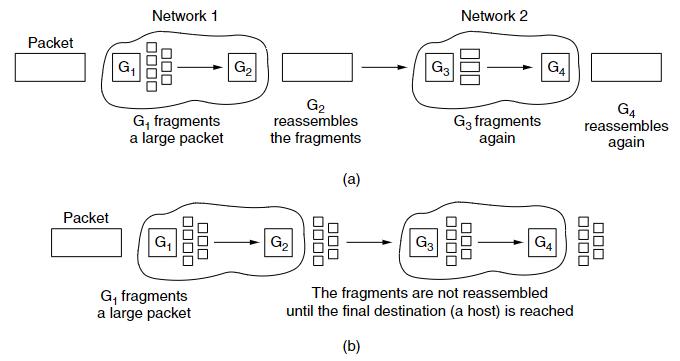
\includegraphics[width=0.42\textwidth]{pic/CN5/recombining the fragments}
    \caption{(a) Transparent fragmentation. (b) Nontransparent fragmentation.}
\end{figure}

e.g. %TODO 94-95

Path MTU discovery

The disadvantage of path MTU discovery is that there may be added startup delays simply to send a packet, more than one round-trip delay may be needed to probe the path

\subsubsection{IPv4 Addressing}
IP 地址有 32 位. 其指向的是一个网络界面, 而不是一台主机. 其是分级的. 其由顶 network portion 与 底 a host portion 组成. IP 也可用 16 进制表示.

% A defining feature of IPv4 is its 32-bit addresses. It is important to note that an IP address does not actually refer to a host. It really refers to a network interface. IP addresses are hierarchical. Each 32-bit address is compromised of a variable-length network portion in the top bits and a host portion in the bottom bits.

Addresses are allocated in blocks called prefixes.
\begin{figure}[!htb]
    \centering
    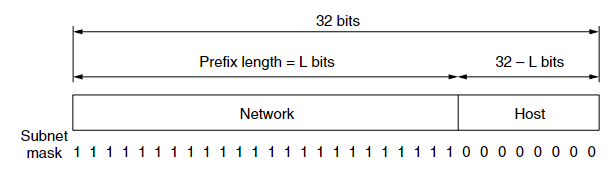
\includegraphics[width=0.42\textwidth]{pic/CN5/An IP prefix and a subnet mask}
    \caption{An IP prefix and a subnet mask}
\end{figure}

\paragraph{IP Prefixes (Network portion)}IP address/length. The /N sometimes known as a subnet mask. 

The key advantage of prefixes is that routers can forward
packets based on only the network portion of the address. 

\paragraph{Subnet}子网个数等于网络中断开路由器后孤岛的个数. 子网 network portion 的地址一致. 将地址块分割成若干部分以供内部用作多个网络. 

\begin{figure}[!htb]
    \centering
    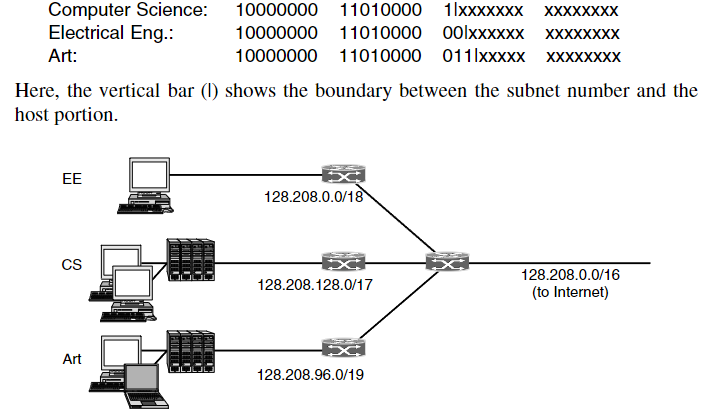
\includegraphics[width=0.42\textwidth]{pic/CN5/Splitting an IP prefix into separate networks with subnetting}
    \caption{Splitting an IP prefix into separate networks with subnetting}
\end{figure}

When a packet comes into the main router, how does the router know which subnet to give it to?
\begin{enumerate}\small
    \item One solution is that for each router to have a table with 65536
    entries telling it which outgoing line to use for each host on
    campus.
    \item The other way is that the router can do this by ANDing the
    destination address with the mask for each subnet and checking
    to see if the result is the corresponding prefix.
\end{enumerate}

\paragraph{IP Address Classes - Historical}Before CIDR, the
network portions of an IP address were constrained to be 8, 16, or 24
bits in length, and addressing scheme known as classful addressing. 

\begin{figure}[!htb]
    \centering
    \includegraphics[width=0.42\textwidth]{pic/CN5/IP address formats}
    \caption{IP address formats}
\end{figure}
分配 IP 地址的机构: the Internet
Corporation for Assigned Names and Numbers (ICANN)
following a hierarchical process

\paragraph{Classless InterDomain Routing(CIDR)} There is still a problem: routing table explosion. 

CIDR solution: 
\begin{itemize}
    \item Subnetting: split IP prefixes
    \item Route aggregation: combine multiple small prefixes into
    a single larger prefix.
\end{itemize}

\paragraph{The Longest Matching Prefix}The rule is that packets are sent in the direction of the most
specific route or the longest matching prefix that has the
fewest IP address

% e.g. 172.16.0.0 ABCD 2000, 4000, 4000, 8000
% 172.16.0.0  | 172.16.7.255  | 172.16.0.0/21
% 172.16.16.0 | 172.16.31.255 | 172.16.16.0/20
% 172.16.32.0 | 172.16.47.255 | 172.16.32.0/20
% 172.16.64.0 | 172.16.95.255 | 172.16.64.0/19

\paragraph{Special IP Addresses}\quad 
\begin{itemize}
    \item 0.0.0.0:  means ``this network'' or ``this host''.
    \item 255.255.255.255: mean all hosts on the indicated network, allows broadcasting
    \item 127.0.0.1 (本机地址)
\end{itemize}

\subsubsection{Protocol} %TODO ???

\paragraph{Network Address Translation(NAT)}
IP addresses are scarce.

Solution:
\begin{enumerate}
    \item DHCP
    \item NAT box (Network Address Translation box)
\end{enumerate}

\begin{figure}[!htb]
    \centering
    \includegraphics[width=0.42\textwidth]{pic/CN5/Network Address Translation}
    \caption{Network Address Translation}
\end{figure}
The NAT translation table includes port numbers as well as IP addresses in the table entries. 通过端口号区分内部的电脑. 

Ports are effectively an extra 16 bits of addressing that identify which process gets which incoming packet. Ports 0-1023 are reserved for well-known services

Problems with NAT:
\begin{itemize}
    \item Port numbers are meant to be used for addressing processes. 
    \item changes the Internet from a connectionless network to a
    peculiar kind of connection-oriented network.
    \item Routers are supposed to process packets only up to layer 3.
    \item violates the most fundamental rule of protocol layering
\end{itemize}

\paragraph{Dynamic Host Configuration Protocol}DHCP is often referred to as a plug-and-play protocol. DHCP is a client-server protocol, each subnet will have a DHCP server. 

In addition to host IP address assignment, DHCP also allows a host
to learn additional information, such as its subnet mask, the
address of its first-hop router (often called the default gateway),
and the address of its local DNS server.

the DHCP protocol is a four-step process:
\begin{enumerate}\small
    \item DHCP server discovery
    \subitem using a DHCP discover message, which a client
    sends within a UDP packet to port 67.
    \subitem broadcast destination IP address of 255.255.255.255 and a “this
    host” source IP address of 0.0.0.0.
    \item DHCP server offer(s)
    \subitem A DHCP server receiving a DHCP discovery message responds to
    the client with a DHCP offer message that is broadcast to all
    nodes on the subnet
    \subitem Several DHCP servers can be present on the subnet, the client may
    choose from among several offers.
    \item DHCP request
    \subitem The newly arriving client will choose from among one or more
    server offers and respond to its selected offer with a DHCP
    request message echoing back the configuration parameters.
    \item DHCP ACK
    \subitem The server responds to the DHCP request message with a DHCP
    ACK message, confirming the requested parameters.
\end{enumerate}
Once the client receives the DHCP ACK, the interaction is
complete and the client can use the DHCP-allocated IP
address for the lease duration. 

\begin{figure}[!htb]
    \centering
    \includegraphics[width=0.309\textwidth]{pic/CN5/DHCP.png}
    \caption{DHCP}
\end{figure}


\subsubsection{IPv6 datagram}
IPv6 uses 128-bit addresses
\begin{figure}[!htb]
    \centering
    \includegraphics[width=0.42\textwidth]{pic/CN5/The IPv6 fixed header }
    \caption{The IPv6 fixed header }
\end{figure}

\begin{enumerate}%TODO 123-124
    \item the Version field (4 bits)
    \item the Difference Services field (8 bits)
    \item the Flow Label field (20 bits)
    \item the Payload length field (16 bits)
    \item the Next Header field (8 bits)
    \item the Hop Limit field (8 bits)
    \item the Source address and Destination address fields (each
    with 128 bits or 16 bytes)
\end{enumerate}

\subsubsection{The IPv6 Address}
Since many addresses will have many zeros inside them,
three optimization have been authorized:
\begin{enumerate}%TODO 125
    \item 
\end{enumerate}

Several Fields in IPv4 are no longer present in the IPv6 datagram
\begin{itemize}
    \item Fragmentation/reassembly
    \item Header checksum
    \item Options
\end{itemize}

Transitioning from IPv4 to IPv6: two approaches
\begin{enumerate}
    \item IPv6-capable nodes is a dual-stack approach, where IPv6
    nodes also have a complete IPv4 implementation
    \item Tunneling. To take the entire IPv6 datagram into the data
    (payload) field of an IPv4 datagram.
\end{enumerate}

Tunneling %TODO 132


\subsection{Control Protocols}

\subsubsection{Internet Control Message Protocol (ICMP)}
The most typical use of ICMP is for error reporting. ICMP is often considered part of IP but architecturally it lies
just above IP, as ICMP messages are carried inside IP
datagrams.

%TODO P138, note 3 3

\paragraph{Use of ICMP --- ``ping''}\quad

\begin{itemize}
    \item ping sends an ICMP
    type 8 code 0 message (echo request) to the
    specified host.
    \item The destination host, seeing the echo request, sends
    back a type 0 code 0 ICMP echo reply.
\end{itemize}

\paragraph{Use of ICMP --- ``Tracert''}Tracert is implemented with ICMP messages,  to determine
the names and addresses of the routers between source and
destination
\begin{enumerate}\small %TODO 142-144
    \item Tracert in the source sends a series of ordinary IP datagrams to
    the destination.
    \item When the nth datagram arrives at the nth router, the nth router
    observes that the TTL of the datagram has just expired.
    \item When this ICMP message arrives back at the source, the source
    obtains the round-trip time from the timer and the name and IP
    address of the nth router from the ICMP message
    \item How does a Tracert source know when to stop sending UDP segments?
\end{enumerate}

\subsubsection{ARP (The Address Resolution Protocol)}
The purpose of the ARP query packet is to query all the other
nodes on the subnet to determine the MAC address corresponding
to the IP address that is being resolved. 

e.g. How a user on host 1 sends a packet to a user on host 2 on
the CS network? %TODO 152-154
\begin{enumerate}
    \item 
\end{enumerate}

\paragraph{Various Optimizations of ARP}\quad %TODO 156-162
\begin{enumerate}
    \item Cache
    \item The default gateway
    \subitem Through the Default Gateway
    \begin{enumerate}
        \item 
    \end{enumerate}
    \item Proxy ARP
\end{enumerate}

\paragraph{ARP vs. DNS}\quad
\begin{itemize}
    \item ARP resolves an IP address to a MAC address only for nodes on
    the same subnet
    \item DNS resolves host names to IP addresses for hosts anywhere in the
    Internet.
\end{itemize}
ARP is probably best considered a protocol that straddles the boundary between the link and network layers

\subsection{Routing Protocols}
A two-level routing algorithm:
\begin{itemize}
    \item Distance vector routing
    \item Link state routing
\end{itemize}
The networks may all use different intradomain protocols, but they must use the same interdomain protocol. 

\subsubsection{The Internet}
In the network layer, the Internet can be viewed as a collection of networks or ASes (Autonomous Systems) that are interconnected. The glue that holds the whole Internet together is the network layer
protocol, IP (Internet Protocol).

\subsubsection{Autonomous System(AS)}
we will examine two intra-AS routing
protocols (RIP and OSPF) and the inter-AS routing
protocol (BGP) that are used in today's Internet

\paragraph{Intra-AS Routing in the Internet: RIP}RIP (Routing Information Protocol) is a distance-vector protocol. 

RIP uses hop count as a cost metric. %TODO 172
\begin{itemize}
    \item 
\end{itemize}

\begin{enumerate}\small
    \item RIP从已配置接口发送整个路由表,该表以广播或组播(Multicast, 目的地址224.0.0.9)的形式周期性向所有节点发送。
    \item “路由更新”定时器规定了周期性广播或组播的频率,缺省值定为30秒。
    \item 如果达到无效(invalid)超时时间(缺省为180秒)时,路由器仍未收到某路由器的路由更新信息,将把该条路由标记为无效,认为不可达,标记为无效的方式就是将跳数设定为16。
    \item 被标记为不可达的路由仍将保存在路由表里,直到清除定时器超时后,才被清除掉,清除定时器的缺省值为240秒。
    \item 当某一路由项RI包含的目的网络变成不可达到后,该路由项对应的抑制定时器开始计时,在此定时器超时前,即使路由器收到的路由更新指明路由项RI又可达到了,路由项RI仍被本路由器标识为不可到达,只有在抑制定时器超时后,指明路由项RI可到达的路由更新才起作用。抑制定时器的目的在于使路由稳定,不要发生路径摇摆。
\end{enumerate}

\paragraph{OSPF: An Interior Gateway Routing Protocol}% 在实验lab5中讲, 记得搬过来. 
OSPF (Open Shortest Path First,开放式最短路径优先协议). Link state routing. 

The higher data rate, the lower cost of the channel.

\begin{figure}[!htb]
    \centering
    \includegraphics[width=0.309\textwidth]{pic/CN5/OSPF Cost Table}
    \caption{OSPF Cost Table}
\end{figure}

%TODO lab5 15-27, 38

OSPF allows an AS to be divided into numbered areas. An area is a generalization of an individual network. Routers that lie wholly within an area are called internal routers.

Every AS has a backbone area, called area 0. The routers in this area are called backbone routers. All areas are connected to the backbone, possibly by tunnels. 

Each router that is connected to two or more areas is called an area border router (ABR). It must also be part of the backbone. The job of an area border router is to summarize the destinations in one area and to inject this summary into the other areas to which it is connected. This summary includes cost information but not all the details of the topology within an area. If there is only one border router out of an area, even the summary does not need to be passed. This kind of area is called a stub area.

Each router within an area has the same link state database and runs the same shortest path algorithm.

the designed router and A backup designed router

\subsection{BGP: The Exterior Gateway Routing Protocol}
BGP is an absolutely critical protocol for the Internet --- in essence, it is the protocol that glues the whole thing together.

In BGP, pairs of routers exchange routing information over semipermanent TCP connections using port 179. In BGP, destinations are not hosts but instead are CIDRized prefixes. In BGP, an autonomous system is identified by its globally unique autonomous system number (ASN). In BGP jargon, \textit{a prefix along with its attributes} is called \textbf{a route}. %TODO P185 ebgp and ibgp 

\subsubsection{BGP Route Advertising}
Route advertisements contain \textbf{an IP prefix, AS-path, next hop}. Route advertisements move in the opposite direction to traffic.

\begin{figure}[!htb]
    \centering
    \includegraphics[width=0.42\textwidth]{pic/CN5/Propagation of BGP route advertisements}
    \caption{Propagation of BGP route advertisements}
\end{figure}

TRANSIT service(TR) and PEER service(PE). Note that peering is not transit 

\begin{figure}[!htb]
    \centering
    \includegraphics[width=0.42\textwidth]{pic/CN5/Routing policies between four autonomous systems}
    \caption{Routing policies between four autonomous systems}
\end{figure}

\subsubsection{BGP Policy}
Policy is implemented in two ways:
\begin{enumerate}
    \item Border routers of ISP announce paths only to other
    parties who may use those paths
    \item Border routers of ISP select the best path of the ones they
    hear in any, non-shortest way
\end{enumerate}

\subsection{MPLS}
MPLS (Multiprotocol Label Switching) is perilously close to circuit switching. 
\begin{itemize}
    \item To improve the forwarding speed of IP routers by adopting a key
    concept from the world of virtual-circuit networks: a fixed-length
    label
    \item allowing routers to forward datagrams based on fixed-length
    labels (rather than destination IP addresses)
\end{itemize}

\begin{enumerate}
    \item The 1st question to ask is where does the label go?
    \subitem MPLS falls between the network layer protocol and the data link layer protocol. MPLS is sometimes described as a layer 2.5 protocol. 
    \item the 2nd question is to ask when and how the labels are attached to packets?%TODO 196-198
    \subitem Within the MPLS network, the label is used to forward the packet.
    \begin{figure}[!htb]
        \centering
        \includegraphics[width=0.42\textwidth]{pic/CN5/Forwarding an IP packet through an MPLS network}
        \caption{Forwarding an IP packet through an MPLS network}
    \end{figure}
    \item The final question we will ask is how the label forwarding tables are set up so that packets follow them %TODO P199-200
    \subitem a setup packet is launched into the
    network to create the path and make the forwarding table entries. allocates a label for each
    one and passes the labels to its neighbors. 
\end{enumerate}

\subsection{Internet Multicasting}
IP supports one-to-many communication, or multicasting, using class D IP addresses. 28 bits are available for identifying groups, so over 250 million
groups can exist at the same time.

Some examples of local multicast addresses are:
\begin{itemize}%TODO 201
    \item 
\end{itemize}


    \newpage
\section{Transport Layer}
\subsection{Overview of the transport layer}
Together with the network layer, the transport layer is the heart of the protocol hierarchy. The transport layer provides end-to-end connectivity across the network. 

\begin{figure}[!htb]
    \centering
    \includegraphics[width=0.42\textwidth]{pic/CN6/The network, transport, and application layers}
    \caption{The network, transport, and application layers}
\end{figure}

\subsubsection{The Transport Service}
Two types of transport service
\begin{itemize}
    \item Connection-oriented transport service
    \item Connectionless transport service
\end{itemize}
The transport code runs entirely on the users'machines, but the network layer mostly runs on the routers. The network service is generally unreliable. 

\subsubsection{Transit Units of Different Layers}
\begin{itemize}
    \item Transport layer: segment or TPDU (Transport Protocol Data Unit)
    \item Network layer: packet
    \item Data link layer: frame
    \item Physical layer: bit
\end{itemize}

\begin{figure}[!htb]
    \centering
    \includegraphics[width=0.42\textwidth]{pic/CN6/Nesting of segments, packets, and frames}
    \caption{Nesting of segments, packets, and frames}
\end{figure}

The Internet has two main protocols in the transport layer:
\begin{itemize}
    \item UDP (User Datagram Protocol, connectionless protocol): It does nothing beyond sending packets between applications. It typically runs in the operating system.
    \item TCP (connection-oriented protocol): It does almost everything. It makes connections and adds reliability with retransmission, along with flow control and congestion control.
\end{itemize}

\subsection{The internet transport protocols: UDP}
UDP: connectionless transport protocol. 

\begin{figure}[!htb]
    \centering
    \includegraphics[width=0.42\textwidth]{pic/CN6/The UDP header}
    \caption{The UDP header}
\end{figure}

The two ports serve to identify the endpoints within the source and destination machines

\begin{itemize}
    \item UDP header (8 bytes)
    \begin{itemize}\small
        \item The UDP length field includes the 8-byte header and the data
        \subitem The minimum length is 8 bytes. The maximum length is 65,515 bytes. 
        \item The UDP checksum field (optional) is to provide extra reliability
        \subitem It checksums the header, data, and a conceptual IP pseudoheader
        \subitem The checksum algorithm is simply to add up all the 16-bit words (note here a word = 16 bits = 2 bytes) in one's complement and to take the one's complement of the sum.
    \end{itemize}
    \item The IPv4 pseudoheader
\end{itemize}
\begin{figure}[!htb]
    \centering
    \includegraphics[width=0.42\textwidth]{pic/CN6/The IPv4 pseudoheader included in the UDP checksum.}
    \caption{The IPv4 pseudoheader included in the UDP checksum.}
\end{figure}

What UDP does not do: Flow control, congestion control, or retransmission upon receipt of a bad segment. 

What UDP does do:
\begin{itemize}
    \item To provide an interface to the IP protocol with the added feature of
    demultiplexing multiple processes using the ports.
    \item Optional end-to-end error detection (checksum)
\end{itemize}

The application uses the UDP protocol: 
\begin{itemize}
    \item DNS (Domain Name System, Chapter 7)
    \item SSDP (Simple Service Discovery Protocol)
\end{itemize}

\subsubsection{Real-Time Transport Protocol (RTP)}
It is a transport protocol but just happens to be implemented in the application layer.

Two aspects of real-time transport:
\begin{itemize}
    \item The RTP protocol for transporting audio and video data in packets
    \item How the receiver plays out the audio and video at the right time?
\end{itemize}

\begin{figure}[!htb]
    \centering
    \includegraphics[width=0.42\textwidth]{pic/CN6/RTP.png}
    \caption{(a) The position of RTP in the protocol stack. (b) Packet nesting.}
\end{figure}

The basic function of RTP is to multiplex several real-time data streams onto a single stream of UDP packets

\begin{figure}[!htb]
    \centering
    \includegraphics[width=0.42\textwidth]{pic/CN6/The RTP header}
    \caption{The RTP header}
\end{figure}
It consists of three 32- bit words and potentially some extensions
\begin{itemize}\small
    \item The Version field: 2
    \item The P bit indicates that the packet has been padded to a multiple of 4 bytes. The last padding byte tells how many bytes were added.
    \item The X bit indicates that an extension header is present.
    \item The CC field tells how many contributing sources are present, from 0 to 15.
    \item The M bit field is an application-specific marker bit.
    \item The Payload type field tells which encoding algorithm has been used.
    \item The Sequence number is just a counter that is incremented on each RTP packet sent. It is used to detect lost packets.
    \item The Timestamp is produced by the stream’s source to note when the 1st sample in the packet was made.
    \item The Synchronization source identifier tells which stream the packet belongs to.
    \item The Contributing source identifier, if any, are used when mixers are present in the studio.
\end{itemize}

\subsubsection{RTCP}
The RTCP (Real-time Transport Control Protocol) is a little sister protocol of RTP

Playout with Buffering and Jitter Control
\begin{figure}[!htb]
    \centering
    \includegraphics[width=0.42\textwidth]{pic/CN6/Smoothing the output stream by buffering packets}
    \caption{Smoothing the output stream by buffering packets}
\end{figure}

\subsection{The internet transport protocols: TCP}
TCP (Transmission Control Protocol) was designed to provide a reliable end-to-end byte stream over an unreliable internetwork. 

An internetwork may have wildly different topologies, bandwidths, delays, packet sizes, and other parameters in different parts.

\subsubsection{The TCP Service Model}
TCP service is obtained by both the sender and the receiver creating end points, called sockets. Each socket has a socket number (address) consisting of the IP addressing of the host and a 16-bit number local to that host, called a port.

All TCP connections are full duplex and point-to-point. TCP does not support multicasting and broadcasting. 

A TCP connection is a byte stream, not a message stream. (报文粘连问题)
\begin{figure}[!htb]
    \centering
    \includegraphics[width=0.42\textwidth]{pic/CN6/TCP connection is a byte stream}
    \caption{ (a) Four 512-byte segments sent as separate IP datagrams. (b) The 2048 bytes of data delivered to the application in a single READ call.}
\end{figure}

When an application passes data to TCP, TCP may send it immediately or buffer it.
\begin{itemize}
    \item PUSH flag: send immediately
    \item URGENT flag: high priority
\end{itemize}

\begin{figure}[!htb]
    \centering
    \includegraphics[width=0.309\textwidth]{pic/CN6/Some assigned ports}
    \caption{Some assigned ports}
\end{figure}

The TCP Protocol includes: a fixed 20-byte header + <optional> + <0-N data bytes>. 

The form of data exchange: segment. 

The basic TCP protocol: the sliding window protocol with dynamic window size. 

There are many problems to solve:
\begin{enumerate}
    \item Segment can arrive out of order
    \item Segments can also be delayed
\end{enumerate}

\subsubsection{The TCP Segment Header}
A key feature of TCP, and one that dominants the protocol design, is that every byte on a TCP connection has its own 32-bit sequence number. Every segment begins with a fixed-format, 20-byte header. 

Segments without any data are legal and are commonly used for acknowledgements and control messages.

\begin{figure}[!htb]
    \centering
    \includegraphics[width=0.42\textwidth]{pic/CN6/The TCP header}
    \caption{The TCP header}
\end{figure}

\begin{enumerate}
    \item The Source port (16 bits) and Destination port (16 bits)
    \subitem The connection identifier is a 5 tuple because it consists of five pieces of information: the protocol (TCP), source IP, and source port, and destination IP and destination port.
    \item The Sequence number (32 bits) and Acknowledgement number (32 bits) fields
    \subitem The Acknowledgement number specifies the next in-order byte expected, not the last byte correctly received.
    \subitem It is a cumulative acknowledgement because it summarizes the
    received data with a single number.
    \item The TCP header length (4 bits): because of the Options field. 
    \item The not used 4-bit field
    \item eight 1-bit fields (ack, syn, fin is important)
    \begin{itemize}\small
        \item CWR and ECE are used to signal congestion when ECN (Explicit Congestion Notification) is used.
        \subitem ECE is set to signal an ECN-Echo to a TCP sender
        \subitem CWR is set to signal Congestion Window Reduced from the TCP sender
        \item URG is set to 1 if the Urgent pointer is in use.
        \subitem The Urgent pointer is used to indicate which urgent data are to be found
        \item The ACK bit is set to 1 to indicate that the Acknowledgement number is valid
        \item The PSH bit indicates PUSHed data
        \item The RST bit is used to abruptly reset a connection
        \item The SYN bit is used to establish connections
        \begin{itemize}\scriptsize
            \item The connection request has SYN = 1 and ACK= 0
            \item SYN = 1 and ACK = 1: the connection reply does bear an acknowledgement.
        \end{itemize}
        \item The FIN bit is used to release a connection. 
        \subitem Both SYN and FIN segments have sequence numbers and are thus guaranteed to be processed in the corrected order.
    \end{itemize}
    \item The Window size field (16 bits) tells how many bytes
    may be sent starting at the byte acknowledged
    \subitem A window size field of 0 is legal, would like no more data for the moment. 
    \item Checksum (16 bits).  It checksum the header, the data and a conceptual pseudoheader. 
    \begin{figure}[!htb]
        \centering
        \includegraphics[width=0.42\textwidth]{pic/CN6/The pseudoheader of TCP}
        \caption{The pseudoheader of TCP}
    \end{figure}
    \item The Options field. may extended to 40 bytes to accommodate the longest TCP header 
    \begin{itemize}
        \item MSS(Maximum Segment Size), it defaults to a 536-byte load.
        \item The window scale negotiate a window scale factor at the start of a connection
        \item The timestamp 
        \item The SACK (Selective ACKnowledgement), is  used after a packet has been lost but subsequent (or duplicate) data has arrived. 
    \end{itemize}
\end{enumerate}

\subsubsection{TCP Connection Establishment}
Three Way Handshake
\begin{figure}[!htb]
    \centering
    \includegraphics[width=0.42\textwidth]{pic/CN6/TCP Connection Establishment}
    \caption{(a) TCP connection establishment in the normal case. (b) Simultaneous connection establishment on both sides.}
\end{figure}

\begin{enumerate}
    \item Note that a SYN segment
    consumes 1 byte of sequence
    space so that it can be
    acknowledged unambiguously.
    \item The initial sequence number
    chosen by each host should
    cycle slowly. This rule is to
    protect against delayed
    duplicated packets.    
\end{enumerate}

\begin{enumerate}
    \item SYN --- for establishing a connection
    \subitem Request segment contains the following information in TCP header:
    \begin{enumerate}\scriptsize
        \item Initial sequence number (randomly chosen by the client)
        \item SYN bit set to 1.
        \item Maximum segment size
        \item Receiving window size (the limit of unacknowledged data that can be sent to the client, contained in the window size field)       
    \end{enumerate}
    \item SYN + ACK --- After receiving the request segment
    \subitem Reply segment contains the following information in TCP header:
    \begin{enumerate}\scriptsize
        \item Initial sequence number (randomly chosen by the server)
        \item SYN bit set to 1.
        \item Maximum segment size
        \item Receiving window size
        \item Acknowledgement number
        \item ACK bit set to 1. 
    \end{enumerate}
    \item ACK --- After receiving the reply segment
    \subitem sending a pure acknowledgement. Not necessary. 
\end{enumerate}

\paragraph{Important Points}\quad

\begin{itemize}\small
    \item Connection establishment phase consume 1 sequence number of both sides. But pure acknowledgement do not consume any sequence number. 
    \item Pure acknowledgement for the reply segment is not necessary. Client sending the data packet immediately can be considered as an ack. 
    \item For all the segments except the request segment, ACK bit is always set to 1.
    \item Certain parameters are negotiated during connection establishment. 
    \begin{enumerate}
        \item Window size
        \item Maximum segment size
        \item Timer values
    \end{enumerate}
    \item In any TCP segment
    \begin{itemize}\scriptsize
        \item If SYN bit = 1 and ACK bit = 0, then it must be the request
        segment.
        \item If SYN bit = 1 and ACK bit = 1, then it must be the reply segment.
        \item If SYN bit = 0 and ACK bit = 1, then it can be the pure ACK or segment meant for data transfer.
        \item If SYN bit = 0 and ACK bit = 0, then this combination is not possible.
    \end{itemize}
\end{itemize}

\paragraph{\textbf{SYN Flood} Attack} A malicious sender 发送大量 SYN segments, 但不完成链接.

用 SYN cookies 对抗. 即将 sequence number hash, 这样接受时只需要比对 hash 是否一致. 

\subsubsection{TCP Connection Release}
\begin{figure}[!htb]
    \centering
    \includegraphics[width=0.22\textwidth]{pic/CN6/TCP Connection Release}
    \caption{TCP Connection Release}
\end{figure}

Four TCP segments are needed to release a connection: one FIN and one ACK for each direction. 

\textbf{The Two-army Problem}: 需要知道信号是否送达. 

The following steps are followed in terminating the connection:
\begin{enumerate}\scriptsize %TODO 62-63
    \item For terminating the connection
    \item after receiving the FIN segment
    \item After receiving the acknowledgement, client enters the state called FIN\_WAIT\_2. Now
    \item Now suppose server wants to close the connection with the client. For terminating the connection
    \item After receiving the FIN segment
\end{enumerate}

\begin{figure}[!htb]
    \centering
    \includegraphics[width=0.309\textwidth]{pic/CN6/The states used in the TCP connection management finite state machine}
    \caption{The states used in the TCP connection management finite state machine}
\end{figure}

\begin{figure}[!htb]
    \centering
    \includegraphics[width=0.42\textwidth]{pic/CN6/TCP connection management finite state machine}
    \caption{TCP connection management finite state machine}
\end{figure}


\subsubsection{TCP Sliding Window}

\begin{figure}[!htb]
    \centering
    \includegraphics[width=0.22\textwidth]{pic/CN6/Window management in TCP}
    \caption{Window management in TCP}
\end{figure}

Example %TODO 70-72
syn + ack 需要占用一个 sequence number, 纯 ack 不用占用. 每个 byte 都有一个对应的 sequence number, 这个 sequence number 也可以携带 ack. 

\begin{figure}[!htb]
    \centering
    \includegraphics[width=0.1\textwidth]{pic/CN6/An Ladder Example}
    \caption{An Ladder Example}
\end{figure}

\begin{figure}[!htb]
    \centering
    \includegraphics[width=0.309\textwidth]{pic/CN6/An Ladder Example2}
    \caption{An Ladder Example}
\end{figure}

%TODO p72
% 2 ack=20001
% 3 seq=20001 ack=5001
% 4 seq=20001 ack=5001
% 5 seq=5001 ack=21001
% 6 seq=21001 ack=5001
% 7 seq=5001 ack=22001
% 8 seq=22001 ack=5001
% 9 seq=5001 ack=23001
% 10 seq=5001 ack=23001
% 11 seq=23001 ack=6001
% 12 seq=6001 ack=23001


When the window is 0, the sender may not normally send segments, with two exceptions:
\begin{enumerate}\scriptsize
    \item Urgent data may be sent, for example, to allow the user to
    kill the process running on the remote machine
    \item The sender may send a 1-byte segment to force the receiver
    to re-announce the next byte expected and the window size.
    This packet is called a window probe
\end{enumerate}

\paragraph{Nagle's Algorithm}To reduce the bandwidth used by a sender that sends multiple short packets. 当有数据要发送, 先发送一个分片, 缓存其他分片, 受到ack 后一次性发送缓存的分片. 但因为缓存, 高交互系统可能造成死锁. 

\paragraph{Clark's Solution} the silly window syndrome: an interactive application on the receiving side reads data only 1 byte at a time. 只有 receiver 有一定比例的 window 可用后再通知 sender. 

\paragraph{The Silly Window Syndrome}The goal is for the sender not to send small segments and the receiver not to ask for them. 


Another issue that the receiver must handle is that segments may arrive out of order. Solution:
\begin{itemize}\scriptsize
    \item The receiver will buffer the data until it can be passed up to the
    application in order
    \item Acknowledgements can be sent only when all the data up to byte
    acknowledged have been received. This is called a cumulative acknowledgement
\end{itemize}

\subsubsection{TCP timer management}
TCP uses multiple timers (at least conceptually) to do its
work.
\begin{itemize}
    \item The RTO (Retransmission TimeOut)
    \subitem How long should the RTO be ? 
    \item The Persistence timer
    \item The Keepalive timer
    \item The one used in TIME WAIT state
\end{itemize}

\paragraph{The RTO (Retransmission TimeOut)}\quad 

\begin{itemize}
    \item set too short, unnecessary retransmissions will occur.
    \item set too long, performance will suffer due to the long retransmission delay whenever a packet is lost
\end{itemize}
Furthermore, the ack arrival can change rapidly within a few seconds as
congestion builds up or is resolved

The solution is to use a dynamic algorithm: 
\begin{itemize}\scriptsize
    \item SRTT (Smoothed Round-Trip Time, Jacobson,1988)
    \subitem Exponentially Weighted Moving Average (EWMA, R is the current
    estimate of the RTT)
    \begin{align*}
        SRTT=\alpha SRTT+(1-\alpha)R 
    \end{align*}
    where $\alpha =7/8$. 
    \item RTTVAR (Round-Trip Time VARiration)
    \subitem To make the timeout value sensitive to the variance in round-trip times as well as the smoothed round-trip time.
    \begin{align*}
        RTTVAR &=\beta RTTVAR +(1-\beta) |SRTT-R|\\
        RTO&=SRTT +4\times RTTVAR\\
        RTO&=\min(1 sec , RTO)
    \end{align*}
    where $\beta=3/4$
\end{itemize}


One problem that occurs with gathering the samples, R, of the round-trip time is what to do when a segment times out and is sent again. 但当接受 ack 时无法确定是从发的 ack 还是先前的 ack. 

Karn's algorithm: 重传的 rtt 不参与更新 rto. 每次失败的重传 timeout doubled. 

\paragraph{the persistent timer}It is designed to prevent the following deadlock %TODO 85

\paragraph{the keepalive timer}看看对方是否下线. 

\paragraph{the TIME WAIT timer}twice the maximum packet lifetime

\subsubsection{TCP Congestion Control}
The network layer 满了只能 dropping packets(丢包). 所以靠 transport layer 解决. In the Internet, TCP plays the main role in controlling congestion, as well as the main role in reliable transport. 

TCP congestion control is based on a AIMD (Additive
Increase Multiplicative Decrease) control law using a
window and with packet loss(丢包) as the binary signal.

TCP maintains a congestion window(the sending window) and a flow control window(the receiving window):
\begin{itemize}
    \item The congestion window size 是指每时 sender 最大发送的字节数. 
    \subitem The corresponding rate = window size/RTT
    \subitem TCP 用 AIMD 调整 congestion window size
    \item The flow control window size 是指每时最大容纳的字节数. Receiver 通过 TCP Header 告知 sender 其 window size. 
    \subitem 发送字节数应该同时小于 两 window size
    \subitem 任意 window size full, TCP 停止传输数据. 
\end{itemize}

All the Internet TCP algorithms assume that lost packets(丢包) are caused by congestion and monitor timeouts. 

During the implementation, we have two important questions:
\begin{enumerate}\scriptsize
    \item The transmission rate of packets which the sender will use
    \subitem ack clock
    \item The size of the congestion window
    \subitem slow start
\end{enumerate}

%TODO 96
The key observation is that ack 到 sender 的 rate 受 slowest link 制约.
The acknowledgements reflect the times at which the packets arrived at
the receiver after crossing the slow link.
This timing is known as an ack clock. It is an essential part of TCP

\begin{figure}[!htb]
    \centering
    \includegraphics[width=0.42\textwidth]{pic/CN6/A burst of packets from a sender and the returning ack clock}
    \caption{A burst of packets from a sender and the returning ack clock}
\end{figure}

\paragraph{TCP Start Problem}We want to quickly near the right rate, $cwnd_{IDEAL}$. 

Slow-Start Solution: Start by doubling cwnd (the congestion window) every RTT. 每收到一个ACK, 就增加一个数据包, 也就是一个变两个. 
\begin{figure}[!htb]
    \centering
    \includegraphics[width=0.309\textwidth]{pic/CN6/Slow-Start Solution}
    \caption{Slow-Start Solution}
\end{figure}

To keep slow start under control, the sender keeps a threshold for the connection called the slow start threshold (sst).
\begin{itemize}
    \item 起始设置为 flow control window size. 
    \item TCP keeps increasing the congestion window in slow start until
    \begin{enumerate}
        \item a timeout occurs (packet loss): sst 降到 congestion window 的一半, 且重启 slow start. 
        \item the congestion window exceeds the slow start threshold: 从 slow start 变为 additive increase (线性)
    \end{enumerate}
\end{itemize}

additive increase: 完成一个完整的RTT, 才增加一个数据包. 

\begin{figure}[!htb]
    \centering
    \includegraphics[width=0.309\textwidth]{pic/CN6/A mix of linear and the multiplication increase}
    \caption{A mix of linear and the multiplication increase}
\end{figure}

\paragraph{Inferring Loss from ACKs}\quad 
\begin{itemize}
    \item TCP uses a cumulative ACK
    \item Duplicate ACKnowledgements gives us hints about what data hasn't arrived
    \begin{itemize}
        \item 告知收到数据包, 但不是期望的
        \item 将三次相同的 ack 当作 loss
        \item 即使计时器没有 timeout, 但也做重传 (Fast Retransmission)
        \item sst 设置为 congestion window/2, slow start 重启
    \end{itemize}
\end{itemize}

\paragraph{Fast Retransmission}It can repair single segment loss quickly, typically before a timeout %TODO 104 + 12.5 钉钉


\paragraph{Fast Recovery}Fast recovery is the heuristic that implements this behavior
\begin{itemize}%TODO 109
    \item pretend further duplicate ACKs are the expected ACKs
    \item duplicate ACKs are counted (including the three that
    triggered fast retransmission) until the number of packets in the
    network has fallen to the new threshold
    \item Reconcile views when the ACK jumps
\end{itemize}


Two larger changes have also affect TCP implementations
\begin{enumerate}
    \item SACK (Selective ACKnowledgements) 
    \begin{figure}[!htb]
        \centering
        \includegraphics[width=0.42\textwidth]{pic/CN6/Selective acknowledgements}
        \caption{Selective acknowledgements}
    \end{figure}
    \item ECN (Explicit Congestion Notification): an IP layer mechanism
    \begin{itemize}
        \item ECE (ECN-Echo): tell the TCP sender to slow down
        \item CWR: The sender tells the receiver that it has heard the signal
    \end{itemize}
\end{enumerate}

TCP Reno, NewReno, and SACK. (笔记中没有前两个版本)
\begin{itemize}\scriptsize
    \item Reno can repair one loss per RTT
    \subitem Multiple losses cause a timeout
    \item NewReno further refines ACK heuristics
    \subitem Repairs multiple losses without timeout
    \subitem SACK (Selective Acknowledgement) is a better idea
\end{itemize}

\subsection{Introduce new transport layer protocols}
\subsubsection{QUIC} 
全称 (Quick UDP Internet Connection), 中文翻译成 ``快速 UDP 互联网连接'', 是由 Google 提出的使用 UDP 进行多路并发传输的协议. 

%TODO 自己去看 120- 

\begin{enumerate}
    \item Low latency to establish connection
    \item Improved Congestion Control Scheme
    \item reliable transmission based on monotonically increased packed number. 
    \subitem Stream offset
    \item removal of the ``Head-of-Line blocking'' (HOL blocking) problem (队头阻塞问题)
    \item 连接迁移
\end{enumerate}

\subsubsection{BBR} 
(Congestion Control based on Bottleneck Bandwidth)

%TODO 自己去看 130-

现在丢包与拥塞不再等价了. 

A full-duplex TCP connection has exactly one slowest link or bottleneck in each direction. The bottleneck is important because It determines the connection's maximum data-delivery rate. 

Two physical constraints, RTprop (round-trip propagation time) and BtlBw (Bottleneck Bandwidth), bounds transport performance. If the network path were a physical pipe, Rtprop would be its length and BtlBW its minimum diameter. 

\begin{figure}[!htb]
    \centering
    \includegraphics[width=0.309\textwidth]{pic/CN6/bbr.png}
    \caption{RTT and delivery rate variration with the amount of data inflight}
\end{figure}

data in flight (data sent but not yet acknowledged) = BtlBw $\times$ Rtprop

Bandwidth-delay product (BDP) is a measurement of how many bits can fill up a network link

Little's Result:
\begin{align*}
    \bar{N}=\lambda T
\end{align*}
\begin{itemize}
    \item $\bar{N}$ is the data in flight in the network
    \item $T$ RTT
    \item $\lambda$ the delivery rate
\end{itemize}

\begin{align*}
    T&=\frac{\bar{N}}{\lambda}=\frac{\bar{N}}{BtlBw}=RTT\\
    \lambda&=\frac{\bar{N}}{T}=\frac{\bar{N}}{RTprop}
\end{align*}

Rtprop and BtlBw obey an uncertainty principle: whenever one can measured, the other cannot.

Characterizing the bottleneck:
\begin{itemize}
    \item Rate balance
    \item Full pipe
    \item BtlBw and RTprop vary over the life of a connection, so they must be continuously estimated
\end{itemize}
    \newpage
\section{Application Layer}
\subsection{Overview of application layer}
Builds distributed ``network services'' (DNS, Web) on transport services

\begin{figure}[!htb]
    \centering
    \includegraphics[width=0.42\textwidth]{pic/CN7/Presentation Layers}
    \caption{Presentation Layers}
\end{figure}

\subsubsection{Applications and Application Level Protocols}
The three concepts:
\begin{itemize}
    \item Service model
    \item Protocol
    \item Interface
\end{itemize}

Network application contains Client site, Server site, Application level protocol

\subsubsection{Parameters}
\begin{itemize}
    \item Data Loss
    \item Bandwidth
    \item Timing
\end{itemize}

\subsection{Important application layer protocols}

\subsubsection{DNS (Domain Name System)}
decouple machines names from machine addresses. 

The essence of DNS is the invention of a hierarchical, domain-based naming scheme and a distributed database system for implementing converting the machine names to network addresses. an application program calls a library procedure called the resolver. 

The query and response messages are sent as UDP packets. (现在不一定了, 不过书上是这样写的, 考试要这样答)

Why Not Centric:
\begin{itemize}
    \item Single point of failure
    \item Traffic volume
    \item Distant name server means slow response
    \item Scalability
\end{itemize}

\begin{figure}[!htb]
    \centering
    \includegraphics[width=0.42\textwidth]{pic/CN7/Portion of the hierarchy of DNS servers}
    \caption{Portion of the hierarchy of DNS servers}
\end{figure}


\paragraph{Root Nameservers}Root (dot) is served by 13 server names
\begin{itemize}
    \item a.root-servers.net to m.root-servers.net
    \item Each ``server'' is actually a cluster of replicated servers, for both security and reliability purposes
\end{itemize}

\begin{figure}[!htb]
    \centering
    \includegraphics[width=0.42\textwidth]{pic/CN7/A portion of the Internet domain name space.}
    \caption{A portion of the Internet domain name space.}
\end{figure}

TLDs (Top-Level Domains) Run by ICANN. 

\paragraph{DNS Zones}Each zone has one or more nameservers to contact for
information about it.

\paragraph{Domain Resource Records}The primary function of DNS is to map domain names onto resource records.

A resource record is a five-tuple. The format is as follows:
\begin{itemize}
    \item Domain name: This field is thus the primary search key used to satisfy queries
    \item Time to live: how stable the record is. 
    \item Class: For Internet information, it is always IN
    \item Type
    \begin{figure}[!htb]
        \centering
        \includegraphics[width=0.42\textwidth]{pic/CN7/The principal DNS resource record types.}
        \caption{The principal DNS resource record types.}
    \end{figure}
    \begin{itemize}\scriptsize
        \item An SOA record provides the name of the primary source of information about the name server's zone.
        \item A: 32-bit IPv4 address
        \item AAAA: 128-bit IPv6 address
        \item MX: it specifies the name of the host prepared to accept email for the specific domain
        \item NS: a name server
        \item CNAME: ppt 参考文献 [7]
        \item PTR: allow lookups of the IP address and return the name of the corresponding machine. -- reverse lookups
        \item SRV: a newer type of record that allows a host to be identified for a given service in a domain. 
        \item SPF: This helps receiving machines check that mail is valid.
        \item TXT: 
    \end{itemize}
    \item Value
\end{itemize}

\paragraph{DNS Resolution}DNS protocol lets a host resolve any host name (domain) to IP address. 

\begin{figure}[!htb]
    \centering
    \includegraphics[width=0.42\textwidth]{pic/CN7/Example of a resolver looking up a remote name in 10 steps.}
    \caption{Example of a resolver looking up a remote name in 10 steps.}
\end{figure}

\paragraph{Iterative vs. Recursive Queries}\quad
\begin{itemize}\small
    \item Recursive query: Nameserver completes resolution and returns the final answer (客户端 -- 本地 DNS 服务器)
    \item Iterative query: Nameserver returns the answer or who to contact next for the answer (本地 DNS 服务器 -- 外网)
\end{itemize}

\paragraph{DNS Caching vs. Freshness}Information is cached between 5 minutes and 72 hours

\paragraph{Local Nameservers}Local nameservers typically run by IT

\paragraph{Name Servers}There are 13 root DNS servers. Most of the root servers are
present in multiple geographical locations and reached using
anycast routing, in which a packet is delivered to the nearest
instance of a destination address.

\paragraph{DNS Protocol}Query and response messages are Built on UDP messages, port 53. Service reliability via replicas. Security is a major issue. 

\paragraph{Security of DNS}\quad
Initially, the transaction ID was only 16 bits. This design choice left DNS vulnerable to a variety attacks including ``cache poisoning attack''. (伪造 DNS)

\begin{figure}[!htb]
    \centering
    \includegraphics[width=0.42\textwidth]{pic/CN7/DNS Header}
    \caption{DNS Header}
\end{figure}

\begin{itemize}
    \item Oblivious DNS
    \item DNSsec
\end{itemize}

\subsubsection{FTP(File Transfer)}
FTP: to transfer files to and from a remote host. 

Steps:
\begin{enumerate}
    \item The user first provides the hostname of the remote host, causing
    the FTP client process in the local host to establish a TCP
    connection with the FTP server process in the remote host.
    \item The user then provides the user identification and password,
    which are sent over the TCP connection as part of FTP commands.
    \item Once the server has authorized the user, the user copies one or
    more files stored in the local file system into the remote file system
    (or vice versa).
\end{enumerate}

FTP uses two parallel TCP connections to transfer a file, a
control connection and a data connection.

\subsubsection{Email(Electronic Mail)}
Email is an asynchronous communication medium

Three major components:
\begin{enumerate}
    \item User agents
    \item Message transfer agents (mail servers)
    \item Simple mail transfer protocol: SMTP
\end{enumerate}

\begin{figure}[!htb]
    \centering
    \includegraphics[width=0.42\textwidth]{pic/CN7/Architecture of the email system.}
    \caption{Architecture of the email system.}
\end{figure}

\paragraph{SMTP} is the principal application layer protocol for Internet electronic mail

\paragraph{MIME}The Multimedia Internet Mail Extension

\paragraph{Mail Access Protocols}SMTP has been designed for pushing email form one host to another. obtaining the messages is a pull operation,
whereas SMTP is a push protocol

Final Delivery:
\begin{itemize}
    \item POP
    \item IMAP
    \item HTTP
\end{itemize}

\subsubsection{HTTP(The HyperText Transfer Protocol)}
The HTTP, the Web's application-layer protocol, is at the heart of the
Web.

HTTP is a simple request-response protocol that normally runs over
TCP. HTTP has nothing to do with how a Web page is interpreted by a client.


Web page as a set of related Web resources  The content from these different servers is integrated for display by the browser.

HTTP is a request/response protocol for fetching Web resources

\paragraph{Fetching a Web page with HTTP}\quad
the Client Side

Steps:
\begin{enumerate}
    \item Resolve the server to IP address (DNS)
    \item Set up TCP connection to the server
    \item Send HTTP request for the page
    \item (Await HTTP response for the page)
    \item Execute / fetch embedded resources /render (不只是展示网页中内容,可能还要运行程序等。)
    \item Clean up an idle TCP connections
\end{enumerate}

The Server Side

Steps:
\begin{enumerate}
    \item Accept a TCP connection from a client (a browser).
    \item Get the path to the page, which is the name of the file requested.
    \item Get the file (from disk).
    \item Send the contents of the file to the client.
    \item Release the TCP connection.
\end{enumerate}

\paragraph{Cookies}It remembers stateful information for the stateless HTTP protocol

A cookie may contain up to five fields:
\begin{enumerate}
    \item The Domain tells where the cookie came from
    \item The Path is a path in the server’s directory structure that identifies
    which parts of the server’s file tree may use the cookie.
    \item The Content field is where the cookie’s content is stored.
    \item The Expires field specifies when the cookie expires
    \item The Secure field can be sent to indicate that the browser may only
    return the cookie to a server using a secure transport. This feature
    is used for e-commerce.
\end{enumerate}

%TODO ?-112

\paragraph{HTTP Message Format}\quad %TODO 113

Request

Request Headers

Example

Response

Example

\paragraph{html}需要记 html 一些语法. %TODO 148

css


\paragraph{Dynamic Web Pages}也会考
    \newpage
\section{Network Security}
Basic knowledge
\subsection{Cryptography}
\subsubsection{Kerckhoff's principle}
All algorithms must be public; only the keys are secret.

\subsubsection{Substitution ciphers}
In a substitution cipher, each letter or group of letters is replaced by another letter or group of letters to disguise it.

The basic attack takes advantage of the statistical properties of natural languages.

\subsubsection{Transposition ciphers}
Transposition ciphers, in contrast, reorder the letters but do not disguise them. The cipher is keyed by a word or phrase not containing any repeated letters.

To break a transposition cipher, the cryptanalyst must 
\begin{enumerate}
    \item first be aware that he is dealing with a transposition cipher.
    \item The next step is to make the guess at the number of columns (the key length).
    \item The remaining step is to order the columns.
\end{enumerate}


\subsubsection{One-time pads}
First choose a random bit string as the key. Then convert the plaintext
into a bit string, for example, by using its ASCII representation.
Finally, compute the XOR of these two strings, bit by bit.

The reason derives from information theory: there is simply no
information in the message because all possible plaintexts of the given
length are equally likely.

% \subsubsection{Quantum cryptograph}
\subsubsection{Two fundamental cryptographic principles}
\begin{enumerate}
    \item All the encrypted messages must contain some redundancy.
    \item Measures must be taken to ensure that each message received can be verified as being fresh.
\end{enumerate}

\subsection{Symmetric-key algorithms}
In symmetric-key algorithms, they use the same key for encryption and decryption.


\subsubsection{DES}
要经历 19 个阶段. 

\subsubsection{Triple DES}
whitening, 不确定性达到最大值. 

\subsubsection{Rijndael}

很重要, 但不讲了.jpg

\subsection{Public-key algorithms}

These requirements can be stated simply as follows:
\begin{enumerate}
    \item $D(E(P))=P$
    \item It is exceedingly difficult to deduce $D$ from $E$.
    \item $E$ cannot be broken by a chosen plaintext attack.
\end{enumerate}

Public-key cryptography requires each user to have two keys: a public key, used by the entire world for encrypting message to be sent to that user, and a private key, which the user needs for decrypting messages.

\subsubsection{RSA}%TODO 33-42

\subsection{Digital Signatures}
The authenticity of many legal, financial, and other
documents is determined by the presence or absence of an
authorized handwritten signature.

The basic requirements of digital signatures:
\begin{enumerate}
    \item The receiver can verify the claimed identity of the sender.
    \item The sender cannot later repudiate the contents of the message.
    \item The receiver cannot possibly have concocted the message
    himself.
\end{enumerate}

\subsubsection{Symmetric-Key Signatures}


Replay Attack


\subsubsection{Public-Key Signatures}


\subsubsection{Message Digests}
One criticism of signature methods is that they often couple two
distinct functions: authentication and secrecy. 


SHA-1 and SHA-2


\subsubsection{The Birthday Attack}
The birthday attack is that with two different plaintexts, but
have the same message digests.


\subsection{Management of public keys}
\subsubsection{Certificates}

\subsubsection{Public Key Infrastructures}

    \newpage\
\section{复习}

\end{document}